\chapter{Validation}

\section{Linear elasticity solver validation and verification using method of manufactured solutions}
The main aim of this write-up is to develop and implement the method of manufactured solutions (MMS) within the field of linear elasticity. A FEM solver is developed for solving linear elasticity problems. Within this note MMS is applied to verify and validate this solver.\\

	\noindent\textbf{Mathematical typesetting conventions}\\\\
	\noindent Unless specified, the mathematical typesetting conventions are as follows.\\
	\begin{table}[h]
		\centering
			\begin{tabular}{p{.3\textwidth}p{.2\textwidth}p{.3\textwidth} }
			\hline
			Typesetting &Example&Description\\
			\hline
			Bold uppercase & $\bA,\bM$& Matrices\\
			Bold lowercase & $\bx,\bb,\bff$& Vector\\
			Lowercase Greek   & $\alpha,\beta,\lambda$ & Scalars\\
			Lowercase Roman   & $\textsl{g}$ & Scalars\\			
			Bold Greek   & $\sig,\eps$ & Tensor\\
			Blackboard bold style   & $\mathbb{R}$ & Number set\\												
			\hline
		\end{tabular}
	\end{table}
	

\subsection{Introduction}
	
In order to use the developed FEM solver to predict outcomes from previously unforeseen situations in linear elasticity, it is important to validate and verify the proposed solver. In other words, it is important to build trust on the solvers reliability and know its limits. This can be done by asserting whether the solver is able to reproduce analytical or experimental observations for certain linear elasticity problems. Another way is to compare against results of certain benchmark problems solved with other numerical tools, hence performing cross-validation. Other interesting option is the use of MMS. 

Before progressing further, let us  interpret  what validation and verification means in the context of numerical modeling. Assuming that the mathematical model for a given physics is accurate, the process of \textit{verification}  investigates if an accurate numerical solution to the given mathematical model can be obtained via the numerical method which is being verified. By the process of verification the order of accuracy for the numerical methods can also be calculated. Whereas, the process of \textit{validation} asserts if an appropriate mathematical model has been chosen to describe the physical phenomenon. More elaborate discussions on the process of validation and verification of numerical tools can be found in~\cite{oberkampf2004verification}. 

	 
\subsection{Verification tests with the method of manufactured solutions }
The method of manufactured solutions is used by many numerical communities for solver (code) verification, see for example~\cite{roache1998verification,ecca2007verification,pautz2001verification}. Concerning the solid mechanics solvers, studies such as~\textbf{???} used the method of manufactured solutions for solver verification.

In the method of manufactured solutions, we start with an assumed explicit expression for the solution field (manufactured solution). Then, the solution is substituted  in the  concerned PDE model. This leads to a consistent set of source terms and/or initial conditions and/or boundary conditions. These terms are then used to solve the equation numerically, with the method (solver) that needs to be verified. Finally, by analyzing the error between the numerical solution and the manufactured solution, one can verify if the numerical method works. In addition, by analyzing how the error decreases when finer numerical discretization is considered, one can obtain the order of convergence for the numerical method. 

\subsubsection{Two-dimensional MMS test case}\label{SS:2dMMS}


Let us assume a hypothetical solid material domain ($\Omega\in\mathbb{R}^2$) is acted upon by manufactured forcing vector $\widehat{\bff}=[\widehat{f}_1,\widehat{f}_2]^\top$. This causes the body to deform:
%
\begin{equation}\label{MMS}
\begin{aligned}
&\widehat{u}_1=x^3+x^2y,\\
&\widehat{u}_2=xy^2+x^2y.\\
\end{aligned}
\end{equation}
%
The equation~\eqref{MMS} is our manufactured solution and has been explicitly assumed\footnote{One could chose other expressions, as long as small strain limiting condition is obeyed: $\|\eps\|=\{0.2\times10^{-2};0.5\times10^{-2}\}$}. The task now is to calculate the manufactured forcing vector~$\widehat{\bff}$. In order to do so the following steps are applied.

\begin{itemize}
\item Using \eqref{MMS} for calculating $\nabla\cdot\wbu$:
%
\begin{equation}\label{MMS2}
\begin{aligned}
&\partial_x\wu_1=3x^2+2xy, &~\partial_y\wu_1=x^2,\\
&\partial_x\wu_2=y^2+2xy,  &\partial_y\wu_2=x^2+2xy,
\end{aligned}
\end{equation}
then
\begin{equation}\label{MMS3}
\nabla\cdot\widehat{\mathbf{u}}=\nabla\cdot[\wu_1~~\wu_2]^\top=4(x^2+xy).
\end{equation}
\item Using \eqref{MMS2} for  calculating the manufactured stain tensor $\widehat{\eps}$ components $\widehat{\varepsilon}_{ij}$:
	\begin{equation*}
	\widehat{\varepsilon}_{ij}(\widehat{\bu})=\frac{1}{2}\left( \partial_j \widehat{u}_i+ \partial_i \widehat{u}_j\right),
	\end{equation*}
then
\begin{equation}\label{MMS4}
\begin{aligned}
\we_{11}=3x^2+2xy,\quad\quad\quad\quad &\we_{12}=\frac{1}{2}(x^2+y^2+2xy),\\
\we_{21}=\frac{1}{2}(x^2+y^2+2xy),\quad   &\we_{22}=x^2+2xy.
\end{aligned}
\end{equation}
\item Using \eqref{MMS3} and \eqref{MMS4} for calculating the manufactured stress tensor $\widehat{\sig}$ components $\ws_{ij}$:
\begin{equation*}
\ws_{ij}=\lambda\delta_{ij}\nabla\cdot\wbu+2\mu\we_{ij}(\wbu)
\end{equation*}
then
\begin{equation}
\begin{aligned}
&\ws_{11}=4\lambda(x^2+xy)+2\mu(3x^2+2xy),&\ws_{12}=\mu(x^2+y^2+2xy),\\
&\ws_{21}=\mu(x^2+y^2+2xy),&\ws_{22}=4\lambda(x^2+xy)+2\mu(3x^2+2xy).
\end{aligned}
\end{equation}
\item Finally,  using \eqref{MMS4} for calculating the manufactured force vector $\widehat{\bff}$ components $\widehat{f}_i$:
\begin{equation*}
\begin{aligned}
&\wf_{1}=-\partial_x\ws_{11}-\partial_x\ws_{12},\\
&\wf_{2}=-\partial_x\ws_{21}-\partial_x\ws_{22},
\end{aligned}
\end{equation*}
then
\begin{equation}\label{MMS-force}
\begin{aligned}
&\wf_{1}=-x(8\lambda+14\mu)-y(4\lambda+6\mu),\\
&\wf_{2}=-x(6\lambda+4\mu)-y(2\mu).
\end{aligned}
\end{equation}

Now all we need is a FEM solver that can solve the elasticity system given the manufactured forcing vector \eqref{MMS-force}. Error analysis between the displacement solution vector $\bu^h$ from the FEM solver and the manufactured solution $\wbu$, can then be used to validate and verify the solver. In addition the error analysis will help in assessing the convergence order.  

\end{itemize}

 \begin{figure}[t]
 \centering
 \begin{subfigure}[t]{.23\linewidth}
 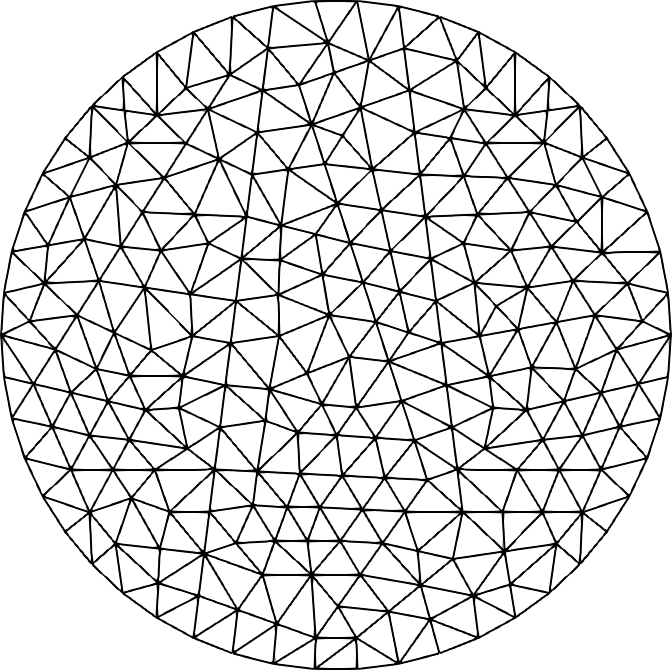
\includegraphics[width=1\textwidth]{./Images/M0.png}
 \caption{Level 1 $\Omega^{0.01}$}
 \end{subfigure}\hfill
  \begin{subfigure}[t]{.23\linewidth}
  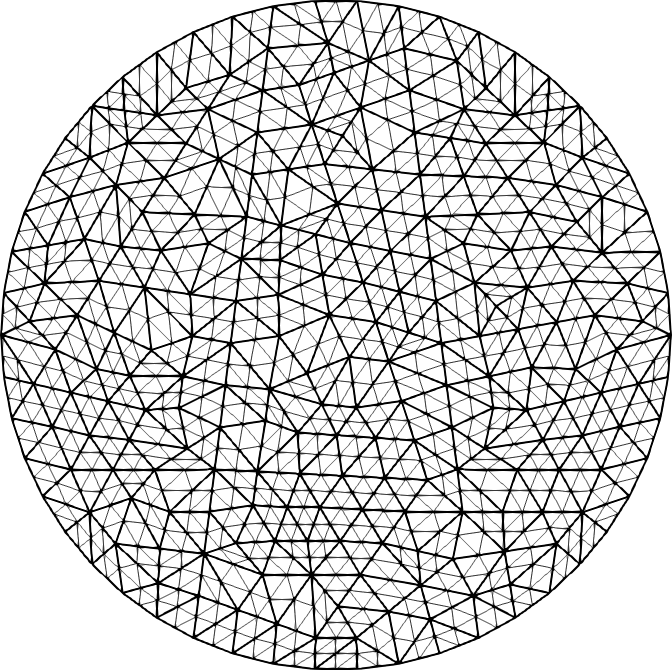
\includegraphics[width=1\textwidth]{./Images/M1.png}
   \caption{Level 2 $\Omega^{0.005}$}
 \end{subfigure}\hfill
  \begin{subfigure}[t]{.23\linewidth}
  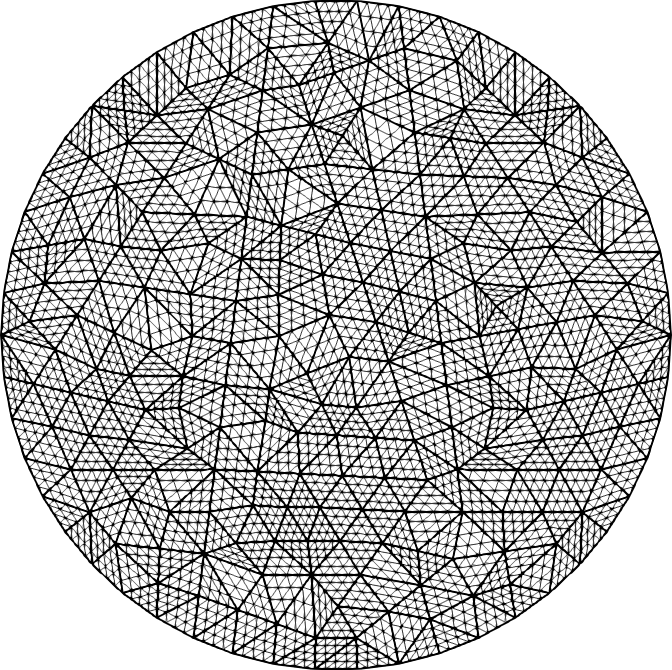
\includegraphics[width=1\textwidth]{./Images/M2.png}
   \caption{Level 3 $\Omega^{0.002}$}
 \end{subfigure}\hfill
  \begin{subfigure}[t]{.23\linewidth}
  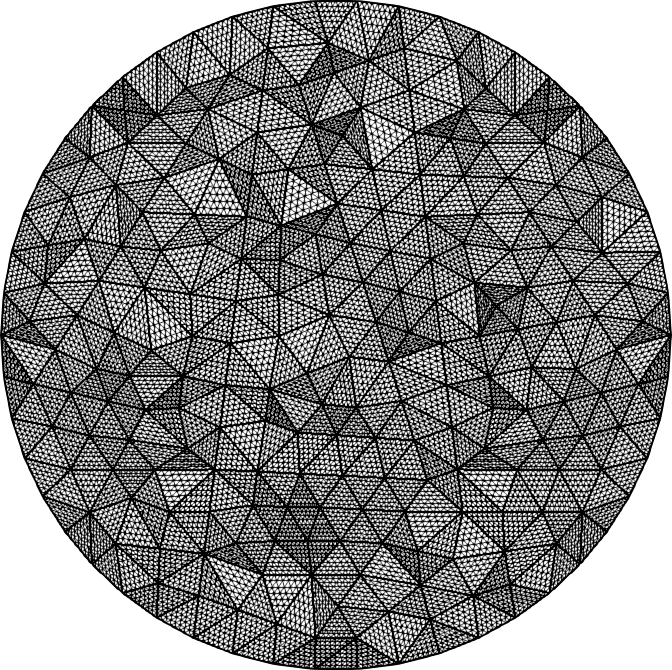
\includegraphics[width=1\textwidth]{./Images/M4.png}
   \caption{Level 4 $\Omega^{0.001}$}
 \end{subfigure}
 \caption{Finite element meshes.}\label{fig:4meshes}
 \end{figure}
	
\subsection{FEM solving model}
Assuming $\Omega^h$ be the bi-dimensional tessellated reference configuration for the hypothetical solid material, or in other words the finite element mesh defined with size parameter~$h$. Finite element variational formulation in the Lagrangian framework for the unknown displacements vector $\bu^h$ then reads, 
	%
	%    
	\begin{equation}\label{varf}
	\left\|\begin{aligned}
	&\text{find}~\bu^h\in[H^1_0(\Omega^h)]^2:\\
	&\int_{\Omega^h}\lambda\nabla\cdot\bu^h\nabla\cdot\bv^h + \int_{\Omega^h}2\mu\boldsymbol\varepsilon(\bu^h):\boldsymbol\varepsilon(\bv^h)+\int_{\Omega^h}\widehat{\bff}\cdot\bv^h=0, \quad\forall\bv^h\in[H^1_0(\Omega^h)]^2,\\
	&\text{given}~\quad\bu^h=\wbu\quad\text{on}\quad\partial\Omega^h_D.
	\end{aligned}\right.
	\end{equation}
	%
Notice in this equation the essential Dirichlet boundary conditions\footnote{For unique solution of the elasticity problem one needs the Dirichlet boundary conditions.} are provided by the known manufactured displacement field $\wbu$ from equation~\eqref{MMS}. Please refer to the other note ``The Krylov subspace based CG solver for linear elasticity", in order to know how the finite element linear system $\bA\bx=\bb$ is assembled and then solved iteratively to derive the displacement field $\wbu: \wbu=\bx^{(m)}$, where $m$ is the converged iteration number for the CG iterative solver. 
	
\begin{table}[htbp]
		\centering
		\begin{tabular}{p{.1\textwidth} p{.17\textwidth}p{.17\textwidth}p{.17\textwidth}p{.17\textwidth} }
			\hline
			 - & Level 1 & Level 2 & Level 3 & Level 4	\\ \hline
			$N_v$ & 244 & 923 & 3,589 & 14,153  \\ 
			$N_e$ & 486 & 1,844 & 7,176  & 28,304  \\ 
			$h_{\text{min}}$ & 0.0102 & 0.0051 & 0.0026 & 0.00013 \\ 
			\hline
		\end{tabular}
\caption{Characteristics of different FEM meshes used for error analysis.
} \label{tab:meshes}
\end{table}	

\subsection{The FEM solver}
To numerically solve equation \eqref{varf}, 
a mixed finite element space based solver is developed using a DSL FreeFem++~\cite{hecht2012new}. The  space discretization kernel of FreeFem++ uses unstructured (triangular or tetrahedral)  mesh inputs. Further, for the linear algebra backend the CG solver provided within FreeFem++. The solver has the capabilities to mix $\mathbb{P}_1$, $\mathbb{P}_2$, and $\mathbb{P}_3$ finite element spaces, for approximating $\bu$. For the sake of simplicity we will only use mixed $\mathbb{P}_1$ spaces, i.e.~in order to solve  \eqref{varf} a mixed finite element space $\boldsymbol{\mathcal{V}}^h:=\mathcal{V}^h\times\mathcal{V}^h$ is defined, such that  $$\bu^h=[u_1^h,u_2^h]^\top\in\boldsymbol{\mathcal{V}}^h\quad\text{and}\quad\bv^h=[v_1^h,v_2^h]^\top\in\boldsymbol{\mathcal{V}}^h.$$ where, $$\mathcal{V}^h({v}^h)=\{{v}^h \in [H^1_0(\Omega^h)], ~{v}^h\in\mathbb{P}_1:{v}^h=\widehat{u} \text{~on~} \partial\Omega^h_D\}.$$

Let us now asses if the developed solver is any good and asses its convergence order. We assume $\Omega$ to be a circle\footnote{Circular domain is  just an assumption, given the mathematics developed in section \ref{SS:2dMMS} one could use any 2D geometry of choice.} of radius 0.1 m and made of a material with modulus of elasticity $E=100$ GPa and Poissons ratio $\nu=0.2$. Let us call this test MMS-test 1. 


\begin{figure}[h]
\centering
\begin{tikzpicture}
\begin{loglogaxis}[
		xmin=0.0008, xmax=.015,
		ymin=1e-9, ymax=1e-5,
		mark repeat={1},
		legend style={at={(.5,1.22)},anchor=north,legend columns=2,font=\fontsize{10}{5}\selectfont},
		legend image post style={scale=.9},
		xtick = {.01, .005, .0025, .00125},
		xticklabels = {0.01, 0.005, 0.0025, 0.00125},
		xlabel={Mesh size $h$},
		ylabel={$L^2$ \& $L^{\infty}$ error norm}
]
		\addplot[line width=1.pt, mark=*, color=blue, dotted, mark size=2pt, mark options={solid}] table[x=h, y=L2u1] {error.dat};\addlegendentry{$L^2 -\mathbb{P}_1 - u_1$};
		\addplot[line width=1.pt, mark=o, color=red, dotted, mark size=3pt, mark options={solid}] table[x=h, y=L2u2] {error.dat};\addlegendentry{$L^{\infty} -\mathbb{P}_1- u_1$};
		\addplot[line width=1.pt, mark=square*, color=blue, dotted, mark size=2pt, mark options={solid}] table[x=h, y=Linfu1] {error.dat};\addlegendentry{$L^2 -\mathbb{P}_1 - u_2$};
		\addplot[line width=1.pt, mark=square, color=red, dotted, mark size=3pt, mark options={solid}] table[x=h, y=Linfu2] {error.dat};\addlegendentry{$L^{\infty} -\mathbb{P}_1- u_2$};
		\logLogSlopeTriangle{0.775}{0.2}{0.25}{1.85}{blue};
		\logLogSlopeTriangle{0.775}{0.2}{.7}{1.89}{red};
       
\end{loglogaxis}
\end{tikzpicture}
\caption{Error between the FEM and manufactured solution. Note that the mesh size $h$ is infact the minimum element size $h_{\min}$ that exists within a mesh $\Omega^{h}$.}\label{fig:error}
\end{figure}

To solve this elasticity problem with FEM, four hierarchical meshes are produced using BMAG: Bidimensional Anisotopic Mesh Generator~\cite{hecht1998bamg}. Hierarchy of refined meshes are obtained by splitting each triangle in the coarse level mesh by four. The split operation is followed to ensure that coarse solutions live in the fine ones. The four hierarchical meshes are presented in figure~\ref{fig:4meshes}. For elaborated characteristics of these meshes refer to table~\ref{tab:meshes}.   

Using the four hierarchical meshes, four simulations of MMS-test 1 were performed. Note, to avoid numerical error discrepancies from the linear solver, the CG iteration was stopped when the relative unpreconditioned residual was lower than $10^{-13}$. The mixed FEM solution for the solver was then compared to the manufactured one and $L^2$ and $L^\infty$ errors were calculated:
\begin{equation}
L^2(\bu)=\left( \int_{\Omega^h} (\wbu-\bu^h)^2\right)^{\frac{1}{2}}\text{ and}
\end{equation}
\begin{equation}
L^\infty(\bu)=\text{max}\left( |\wbu-\bu^h|\right),
\end{equation}
 these are plotted in figure~\ref{fig:error}.  
 
  \begin{figure}[h]
 \centering
 
 \begin{subfigure}[t]{.3\linewidth}
 \centering
  	\begin{minipage}{1\textwidth}
  	\centering
	\begin{tikzpicture}
	\node at (0,0){
\includegraphics[width=.9\textwidth ,height=.07\textwidth]{./Images/scale-h.png}};
	\node at (.45\textwidth,.06\textwidth) {$|$ };
	\node at (-.45\textwidth,.06\textwidth) {$|$ };
	\node at (.4\textwidth,.17\textwidth) { \scriptsize 2.3$\times10^{-12}$};
	\node at (-.35\textwidth,.17\textwidth) { \scriptsize 1.2$\times10^{-3}$};
	\node at (0\textwidth,.09\textwidth) {{\scriptsize Displacement $\|\wbu\|$ }};
	\end{tikzpicture}
 	\end{minipage}\\\vspace{3mm}
 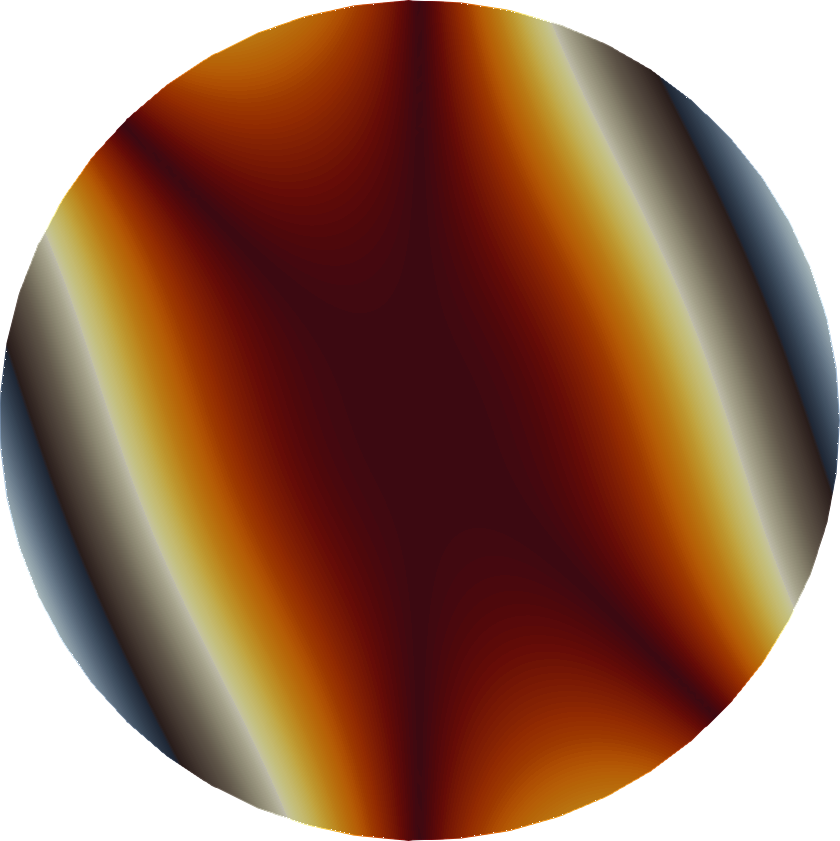
\includegraphics[width=1\textwidth]{./Images/Mms-s8.png}
  \caption{MMS solution.}
 \end{subfigure}\\\vspace{5mm}  
  \begin{subfigure}[t]{.3\linewidth}
   \centering
  	\begin{minipage}{1\textwidth}
  	\centering
	\begin{tikzpicture}
	\node at (0,0){
\includegraphics[width=.9\textwidth ,height=.07\textwidth]{./Images/scale-h.png}};
	\node at (.45\textwidth,.06\textwidth) {$|$ };
	\node at (-.45\textwidth,.06\textwidth) {$|$ };
	\node at (.4\textwidth,.17\textwidth) { \scriptsize 1.2$\times10^{-7}$};
	\node at (-.35\textwidth,.17\textwidth) { \scriptsize 1.2$\times10^{-3}$};
	\node at (0\textwidth,.09\textwidth) {{\scriptsize Displacement $\|\bu\|$ }};
	\end{tikzpicture}
 	\end{minipage}\\\vspace{3mm}   
  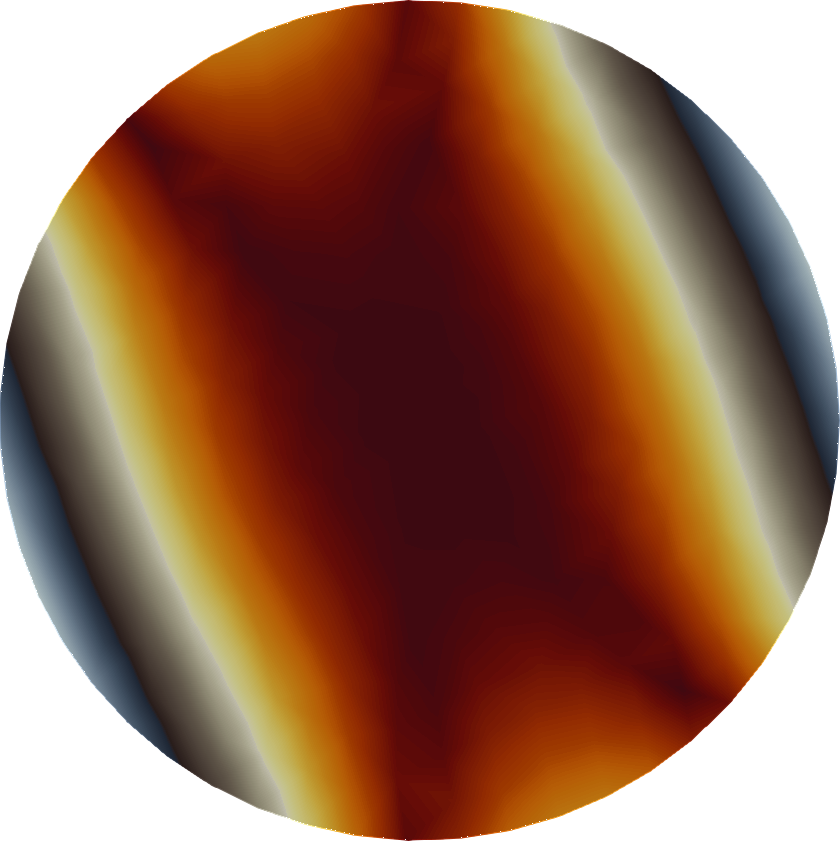
\includegraphics[width=1\textwidth]{./Images/Fem-s1.png}
   \caption{Level 1 FEM solution.}
 \end{subfigure}\hspace{1cm}
   \begin{subfigure}[t]{.3\linewidth}
    \centering
  	\begin{minipage}{1\textwidth}
  	\centering
	\begin{tikzpicture}
	\node at (0,0){
\includegraphics[width=.9\textwidth ,height=.07\textwidth]{./Images/scale-h.png}};
	\node at (.45\textwidth,.06\textwidth) {$|$ };
	\node at (-.45\textwidth,.06\textwidth) {$|$ };
	\node at (.4\textwidth,.17\textwidth) { \scriptsize 2.9$\times10^{-10}$};
	\node at (-.35\textwidth,.17\textwidth) { \scriptsize 1.2$\times10^{-3}$};
	\node at (0\textwidth,.09\textwidth) {{\scriptsize Displacement $\|\bu\|$ }};
	\end{tikzpicture}
 	\end{minipage}\\\vspace{3mm}    
  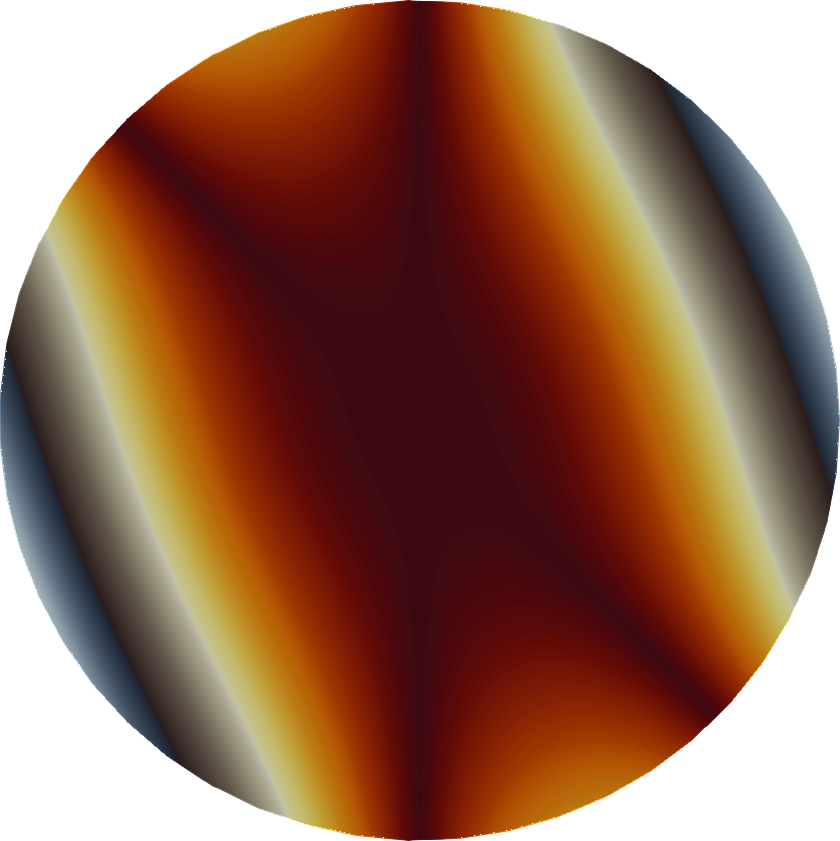
\includegraphics[width=1\textwidth]{./Images/Fem-s8.png}
   \caption{Level 4 FEM solution.}
 \end{subfigure}
 \caption{Displacement field magnitude visualization.}\label{fig:disfiled}
 \end{figure}

Error analysis plot provided in figure~\ref{fig:error} proves that the developed FEM solver has approximately second order convergence rate. More precisely, the $L^2$ error analysis reveled that the FEM solver has the order of  convergences given by 1.85, against theoretical value of 2. Similarly,  the $L^\infty$ error analysis reveled that the FEM solver has the order of  convergences given by 1.89, against theoretical value of 2.  To investigate further the displacement  field magnitudes for the MMS solution and the FEM solutions have been visualized in figure~\ref{fig:disfiled}. Notice how solution improves from the coarsest level mesh (level 1) to the finest one (level 4). It is fair to say that even the coarse level solution is approximating the displacement field well. To investigate further in figure~\ref{fig:errorfiled} the point wise error field is visualized. One can clearly  observe how the error reduces when using ore refined meshes. Moreover, notice that error is zero at the borders, this is due to the fact that all border are Dirichlet borders.  

 
  \begin{figure}
 \centering
  \begin{subfigure}[t]{.3\linewidth}
   \centering
  	\begin{minipage}{1\textwidth}
  	\centering
	\begin{tikzpicture}
	\node at (0,0){
\includegraphics[width=.9\textwidth ,height=.07\textwidth]{./Images/scale-h1.png}};
	\node at (.45\textwidth,.06\textwidth) {$|$ };
	\node at (-.45\textwidth,.06\textwidth) {$|$ };
	\node at (.42\textwidth,.17\textwidth) { \scriptsize 0.0};
	\node at (-.35\textwidth,.17\textwidth) { \scriptsize 3.5$\times10^{-6}$};
	\node at (0\textwidth,.09\textwidth) {{\scriptsize Error $\{L^2\}_i$ }};
	\end{tikzpicture}
 	\end{minipage}\\\vspace{3mm}   
  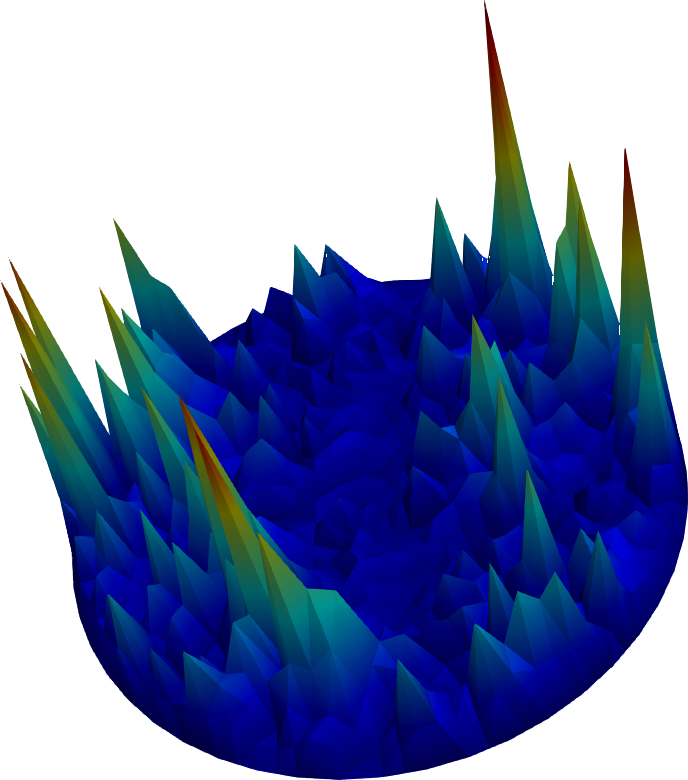
\includegraphics[width=1\textwidth]{./Images/error-s2.png}
   \caption{Level 2 error.}
 \end{subfigure}\hfil
   \begin{subfigure}[t]{.3\linewidth}
    \centering
  	\begin{minipage}{1\textwidth}
  	\centering
	\begin{tikzpicture}
	\node at (0,0){
\includegraphics[width=.9\textwidth ,height=.07\textwidth]{./Images/scale-h1.png}};
	\node at (.45\textwidth,.06\textwidth) {$|$ };
	\node at (-.45\textwidth,.06\textwidth) {$|$ };
	\node at (.42\textwidth,.17\textwidth) { \scriptsize 0.0};
	\node at (-.35\textwidth,.17\textwidth) { \scriptsize 1.4$\times10^{-6}$};
	\node at (0\textwidth,.09\textwidth) {{\scriptsize Error $\{L^2\}_i$ }};
	\end{tikzpicture}
 	\end{minipage}\\\vspace{1.2cm}        
  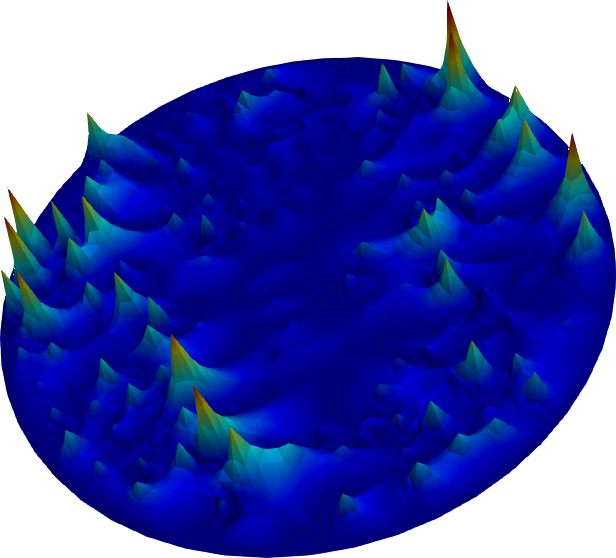
\includegraphics[width=1\textwidth]{./Images/error-s4.png}
   \caption{Level 3 error.}
 \end{subfigure}\hfil
    \begin{subfigure}[t]{.3\linewidth}
    \centering
  	\begin{minipage}{1\textwidth}
  	\centering
	\begin{tikzpicture}
	\node at (0,0){
\includegraphics[width=.9\textwidth ,height=.07\textwidth]{./Images/scale-h1.png}};
	\node at (.45\textwidth,.06\textwidth) {$|$ };
	\node at (-.45\textwidth,.06\textwidth) {$|$ };
	\node at (.42\textwidth,.17\textwidth) { \scriptsize 0.0};
	\node at (-.35\textwidth,.17\textwidth) { \scriptsize 1.6$\times10^{-7}$};
	\node at (0\textwidth,.09\textwidth) {{\scriptsize Error $\{L^2\}_i$ }};
	\end{tikzpicture}
 	\end{minipage}\\\vspace{1.5cm}  
  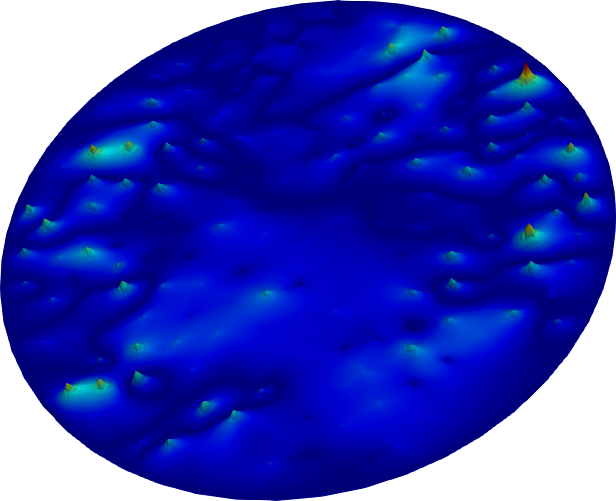
\includegraphics[width=1\textwidth]{./Images/error-s8.png}
   \caption{Level 4 error.}
 \end{subfigure}
 \caption{Warped error field visualization. The warp fields have been magnified a million times for better visualization.}\label{fig:errorfiled}
 \end{figure}
 
 
\section{Damage mechanics solver validation \label{sec:Numerical-benchmarks}}
A commonly used numerical test from literature (see e.g., \cite{Ambati2014,Liu2016,jeong2018phase,Hirshikesh2018} to cite but a few), the two-dimensional (2D) single-edge notched tensile fracture test, is considered as the benchmark problem in this subsection. From here-forth this test is referenced as test~1 in the text. 


\subsubsection{Problem setting \label{sec:2D-problem-statement}}
%
The domain of interest is an initially cracked square plate $(x,y) \in \Omega =[0~\si{\centi\meter},1~\si{\centi\meter}]^2$ (\cref{fig:figcrack-fe-geo-crop-a}). With an initial crack and a constrained bottom edge~$\partial\Omega_{\text{D}}(x,y:y=0)$, the plate  is subject to increasing displacements on its top edge~$\partial\Omega_{\text{D}}(x,y:y=1)$ until the plate fully cracks open.
The initial crack is placed at the center of the plate, i.e., $\partial\Omega_{\text{D}}(x:0 \le x \le 0.5,y:y=0.5)$. These boundary conditions are also illustrated in~\cref{fig:figcrack-fe-geo-crop-a}.
The plate material is characterized by $\lambda=121.15$~\si{\kilo\pascal}, $\mu=80.77$~\si{\kilo\pascal}, and $\bgc=2.7$~\si{\kilo\newton\per\milli\meter}.

Concerning  the  computational specifications of test~1,  the displacement discontinuity  imposed by the initial crack was modeled by nearly overlapping (tolerance $\delta y=10^{-7}$~\si{\meter}) Dirichlet nodes  placed along the cracks edge $\partial\Omega^h_{\text{D}}(x:0 \le x \le 0.5,y:y=0.5\pm\delta y)$ within $\Omega^h$. For illustration proposes,  a coarse grid featuring Dirichlet nodes for the initial crack of test~1 is presented in~\cref{fig:figcrack-fe-geo-crop-b}.
The displacement Dirichlet condition on the top edge is applied with an increment of $\Delta\bar{u}_{2} =1\cdot10^{-5}$~\si{\milli\meter} up to $u_2=5\cdot10^{-3}$~\si{\milli\meter} and $\Delta\bar{u}_{2} =1\cdot10^{-6}$~\si{\milli\meter} up to failure of the specimen. For the lower edge, the constrained displacement Dirichlet conditions $\bar{u}_{1}=\bar{u}_{2}=0$ are applied. Further, for test 1 and for all the simulations that appear in this study, parameter $\kappa$ is set to $1\cdot10^{-6}$ and $l_0$ is assumed equal to $2h$, where $h$ is the characteristic size of the mesh $\Omega^h$.  

The unstructured Delaunay (triangular) meshes generated with Gmsh are used for solving the finite element problem of test~1. To establish mesh convergence, test~1 has been solved multiple times by varying the level of mesh refinements, details of these meshes are provided in~\cref{tab:meshes1}. The hierarchy of mesh refinements were generated by dividing each triangle in $\Omega^h$ into four equal triangles. As such in~\cref{tab:meshes1}, we observe that with every refinement, the mesh size~$h$ halves and the number of triangles quadruple. The initial crack fields for the three mesh refinements (visualized using damage-field $d$) are presented in~\cref{fig:initial-crack}.    %{Since the third order vectorial finite element space $\mathbb{W}^h\in[H^1(\Omega^h)]^3$ is used to approximate the combined displacement and damage variables ($w^h_1,w^h_2,w^h_3$), observe  in~\cref{tab:meshes1}~for a particular mesh level the $\bnd$~(column~5) are thrice the nodes number (column~2).    }

\begin{figure}[tb]
	\centering
	\begin{minipage}[t]{.3\textwidth}
		\centering
		\begin{tikzpicture}
		\node at (0,0) {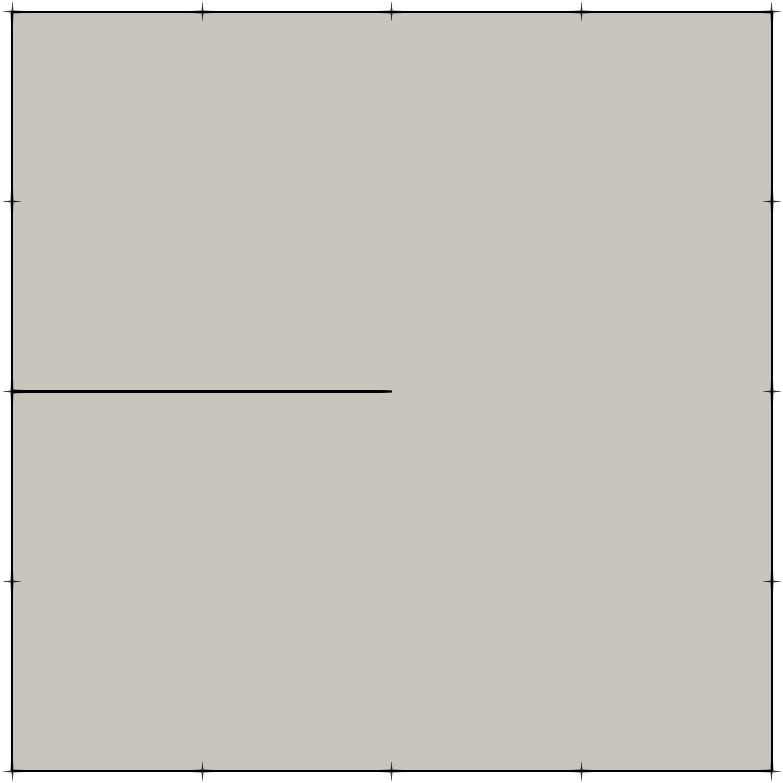
\includegraphics[width=.85\textwidth]{./Images/geo1.png}};
		\node at (-2.,-2.3cm) 		{\small 0};
		\node at (-1.0,-2.3cm) 		{\small 0.25};
		\node at (-0.05,-2.3cm) 	{\small 0.50};
		\node at ( 1.1,-2.3cm) 		{\small 0.75};
		\node at (2.1,-2.3cm) 		{\small 1.0};
		\node at (-2.3,-2.1cm)		{\small 0};
		\node at (-2.45,-1.1cm) 	{\small 0.25};
		\node at (-2.45,0.0cm) 		{\small 0.50};
		\node at (-2.45,1.1cm) 		{\small 0.75};
		\node at (-2.45,2.1cm)      {\small 1.0};
		\node at (0.1,-2.6cm) 		{\small {$x$ axis }};
		\node [rotate=90] at (-3.,0.0cm) 		{\small {$y$ axis }};		
		\node at (1.3,1.3cm) 		{\small $\Omega$};
		\node at (0,-1.68cm)     	{\color{blue}\small $\partial \Omega_\text{D}:u_1=u_2=0$};
		\draw[fill=blue,dotted, fill opacity=.25,draw opacity=0] (-2.1,-2.1cm) rectangle (2.1,-1.95cm);
		\node at (0,1.66cm)      	{\color{magenta}\small $\partial \Omega_\text{D}:u_2=u_2+\Delta u_2$};
		\draw[fill=magenta,dotted, fill opacity=.15,draw opacity=0] (-2.1,2.1cm) rectangle (2.1,1.95cm);
		\node at (-.9,.2cm)      		{\small $\partial \Omega_\text{D}:d=1$};
		\draw[fill=black,dotted, fill opacity=.15,draw opacity=0] (-2.1,-0.05cm) rectangle (0,.05cm);	
		\end{tikzpicture}
		\subcaption{domain~$\Omega$.\label{fig:figcrack-fe-geo-crop-a}}
	\end{minipage}\hspace{.018\textwidth}
	\begin{minipage}[t]{.3\textwidth}
		\centering
		\begin{tikzpicture}
		\node at (0.,0) {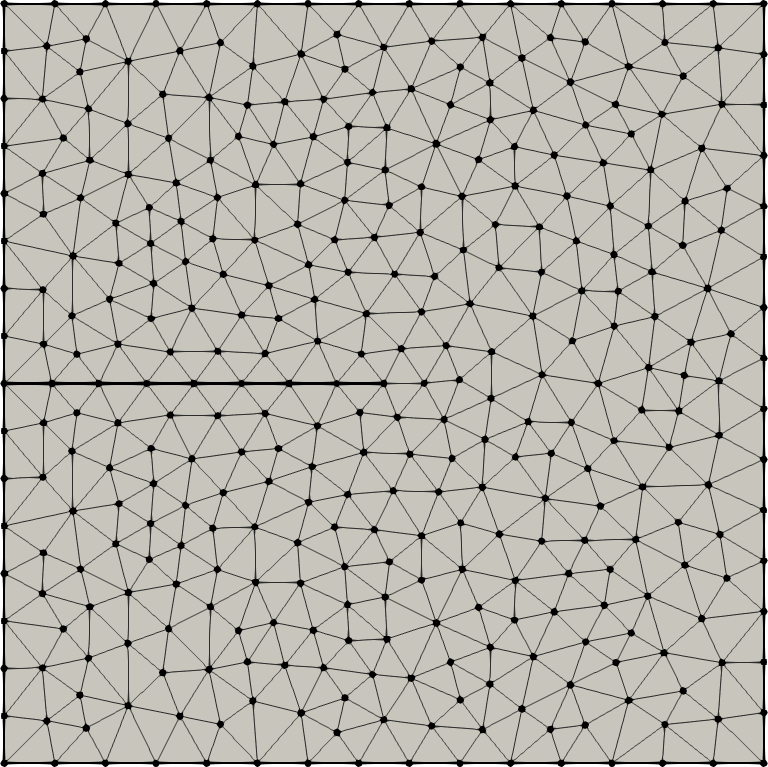
\includegraphics[width=.85\textwidth]{./Images/geo2.png}};
		\node at (0.,-2.7) {~};
		\end{tikzpicture}
		\subcaption{a coarse mesh~$\Omega^h$.\label{fig:figcrack-fe-geo-crop-b}}
	\end{minipage}\hspace{-.02\textwidth}
	\begin{minipage}[t]{.3\textwidth}
		\centering
		\begin{tikzpicture}
		\node at (0.,0) {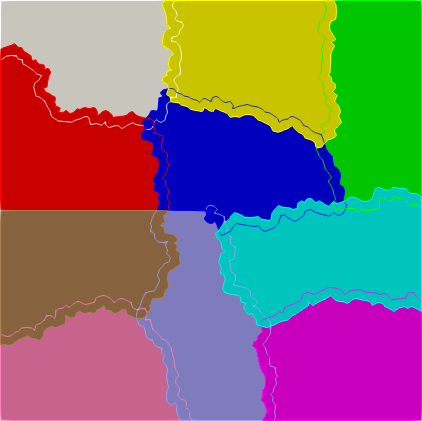
\includegraphics[width=.85\textwidth]{./Images/part-domain-2d.png}};
		\node at (0.,-2.7) {~};
		\end{tikzpicture}
		\subcaption{partitioned mesh~$\{\Omega^h_i\}_{i=1}^{10}$.\label{fig:figcrack-fe-geo-crop-c}}
	\end{minipage}
	\caption{domain~$\Omega$, mesh~$\Omega^h$, and partitioned mesh~$\{\Omega^h_i\}_{i=1}^{10}$~for test~1. (a) also illustrates the boundary conditions applied to test~1. (b) represents a coarse unstructured finite element mesh with `nearly' duplicate Dirichlet nodes for the initial crack.\label{fig:figcrack-fe-geo-crop}}
\end{figure}	

\begin{figure}[tb]
	\centering
	\begin{minipage}[t]{.3\textwidth}
		\centering 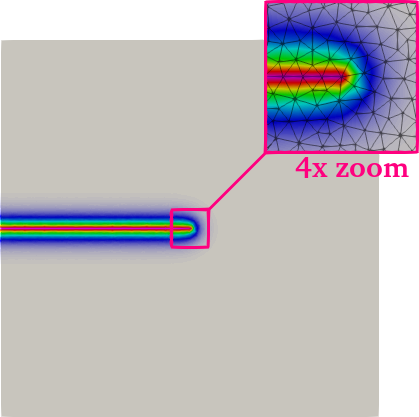
\includegraphics[width=.92\textwidth]{./Images/d-level1.png}
		\subcaption{$d$ at mesh level 1.\label{fig:initial-crack-a}}
	\end{minipage}
	\begin{minipage}[t]{.3\textwidth}
		\centering 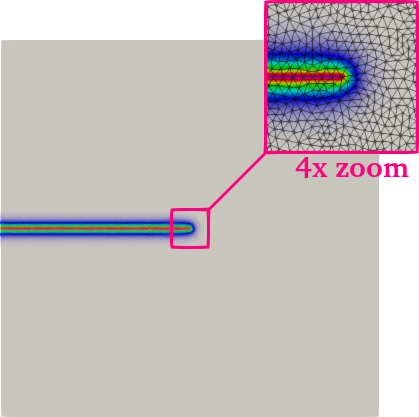
\includegraphics[width=.92\textwidth]{./Images/d-level2.png}
		\subcaption{$d$ at mesh level 2.\label{fig:initial-crack-b}}
	\end{minipage}
	\begin{minipage}[t]{.3\textwidth}
		\centering 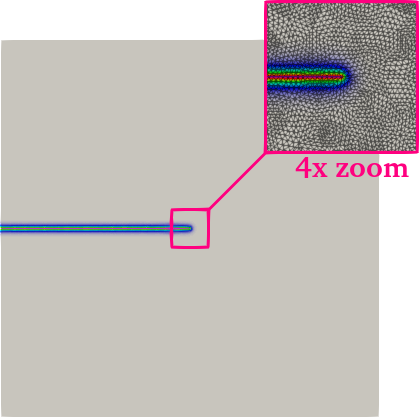
\includegraphics[width=.92\textwidth]{./Images/d-level3.png}
		\subcaption{$d$ at mesh level 3.\label{fig:initial-crack-c}}
	\end{minipage}
	\hspace{-.02\textwidth}
	\begin{minipage}[t]{.02\textwidth}
		\centering
		\begin{tikzpicture}
		\begin{axis}[
		xmin=0, xmax=0.001,
		ymin=0,ymax=1,
		yscale=0.6,
		enlargelimits=false,
		colorbar,
		colormap name=paraviewWR,
		point meta min=0,
		point meta max=1,
		hide axis,
		colorbar style={
			xtick style={draw=none},
			%ytick style={draw=none},
			ytick pos=right,
			tick align = outside,
			title style={yshift=-2.2cm,xshift=0.8cm,rotate=90},
			title={\footnotesize damage-field $d$},
			scaled y ticks = false,
			height = 4cm,
			font = \footnotesize,
			width = 1\textwidth,
			ytick={0,1}
		}
		]	
		\end{axis}
		\node at (0.,-.2) {~};
		\end{tikzpicture}
	\end{minipage}	
	\caption{ initial crack visualization of test 1 via damage-field $d$ at different mesh levels.\label{fig:initial-crack}}
\end{figure}


{
	\pgfplotstableread{
		A			B		C  		D		E		  F						G					H
		%  level~1	4,256	0.0312  6,387	131,193	  17.82\si{\percent}	19.22\si{\percent}		
		level~1	16,384	0.0156  25,059	520,425   17.82\si{\percent}	19.22\si{\percent}  8,353
		level~2	65,536	0.0078	99,267	2,073,033 5.68\si{\percent}		8.12\si{\percent}   33,089
		level~3	262,144	0.0039	395,139	8,274,825 0.45\si{\percent}		0.61\si{\percent}   131,713
		
	}\datatab 
	\begin{table}[tb]\centering
		\caption{characteristics and computational details for the different finite element meshes used for test~1. $E1_{\text{max}(F_y)}$ and $E2_{\text{max}(F_y)}$ are are the the maximum reaction force errors computed against references~\cite{amor2009regularized} and~\cite{Ambati2014}, respectively.\label{tab:meshes1}}
		\pgfplotstabletypeset[
		font=\footnotesize,
		columns={A,H,B,C,D,E,F,G},
		columns/A/.style={column name =mesh,string type,column type = {l}},
		columns/B/.style = {column name =triangles,string type,precision =0,fixed zerofill,column type = {l}},
		columns/C/.style = {column name =$h$,string type,precision =0,fixed zerofill,column type = {l}},
		columns/D/.style = {column name =$\bnd$,string type,fixed zerofill,column type = {l}},
		columns/E/.style = {column name =$\bnz$,string type,fixed zerofill,column type = {l}},
		columns/F/.style = {column name =$E1_{\text{max}(\bl)}$,string type,fixed zerofill,column type = {l}},
		columns/G/.style = {column name =$E2_{\text{max}(\bl)}$,string type,fixed zerofill,column type = {l}},
		columns/H/.style = {column name =nodes,string type,precision =0,fixed zerofill,column type = {l}},						
		every odd row/.style={before row={\rowcolor{white}}},
		every even row/.style={before row={\rowcolor{black!9}}},
		every head row/.style={before row={\midrule},after row=\midrule},
		every last row/.style={after row=\midrule},
		]{\datatab}
	\end{table}
}

\subsubsection{Solver validation \label{sec:solver-validation}}
Using the test~1 we cross-validate and compare our PSD solver (sequential and parallel) against benchmark solutions of this test available in the literature. 
In~\cref{fig:force-comp-2d-tensile-crack}, the top surface reaction force~$F_y$ versus applied displacements is plotted for various mesh refinement levels (detailed in~\cref{tab:meshes1}) and compared to a reference anisotropic phase-field solution from~\cite{amor2009regularized}.

In~\cref{fig:force-comp-2d-tensile-crack}, the mesh convergence is evidenced from the improving PSD solutions (solid lines) towards the reference solution, hence validating  the PSD solver. 
Our computations~(at level~3) are in good agreement with the results provided in~\cite{amor2009regularized}. This simulation was executed using 10 processes on the desktop PC. The parMETIS partitioned mesh with 10 subdomains is presented in~\cref{fig:figcrack-fe-geo-crop-c}.    

To further validate  the PSD solver, we compare the errors in computing the maximum reaction-force $\text{max}(F_y)$ obtained from our solver against two different reference solutions provided in \cite{Ambati2014} and \cite{amor2009regularized}.
The last two columns of~\cref{tab:meshes} enumerate these errors. At finest mesh level~3, these errors decrease down to less than 1\si{\percent}. 
Alongside the plot in~\cref{fig:force-comp-2d-tensile-crack}, four instantaneous snapshots of the calculated damage-fields are presented. These damage-fields are obtained from the  simulation of test~1 at the finest mesh level~3. Damage-field evolution, crack initiation, and propagation can be observed in these snapshots. As expected, under extreme tensile loading, the crack can be seen to travel along  a (almost) straight line dividing the square specimen into two (almost) equal halves. Note that for additional validation, other literature comparative tests (mode I, mode II, and mode III fracture) were also performed but these are not shown here for the sake of conciseness.                        
%
\begin{figure}[tb]
	\centering
	\begin{minipage}{1\textwidth}
		\centering
		\begin{tikzpicture}
		\node at (-0cm,0) {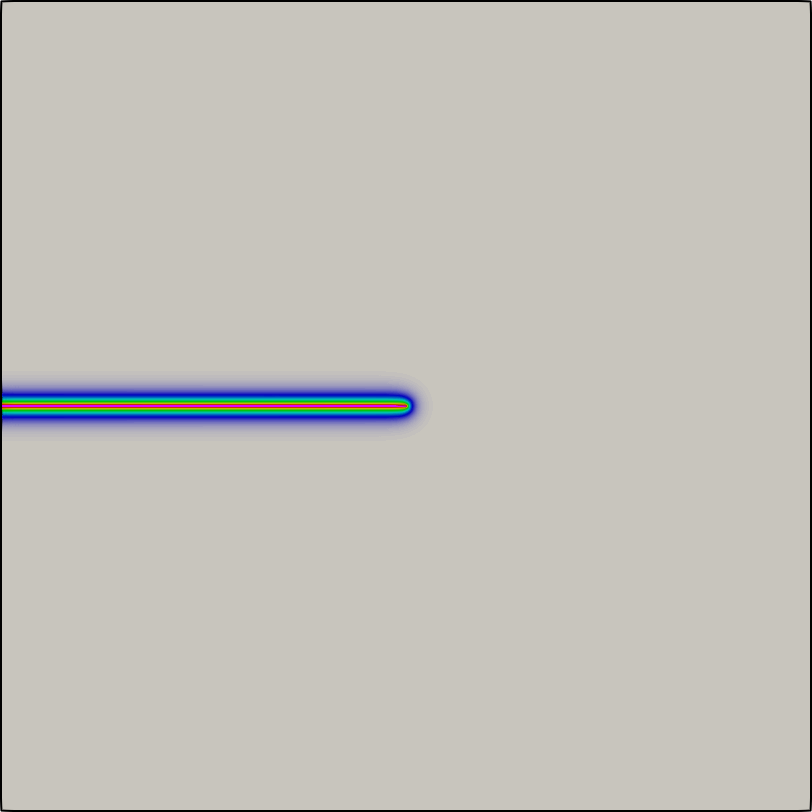
\includegraphics[scale=.1]{./Images/t0-crack.png}};
		\node at (-0cm,0.5cm) {\scriptsize \color{black}crack~tip~(0.5,0.5)};
		\node at (-0cm,3.25cm){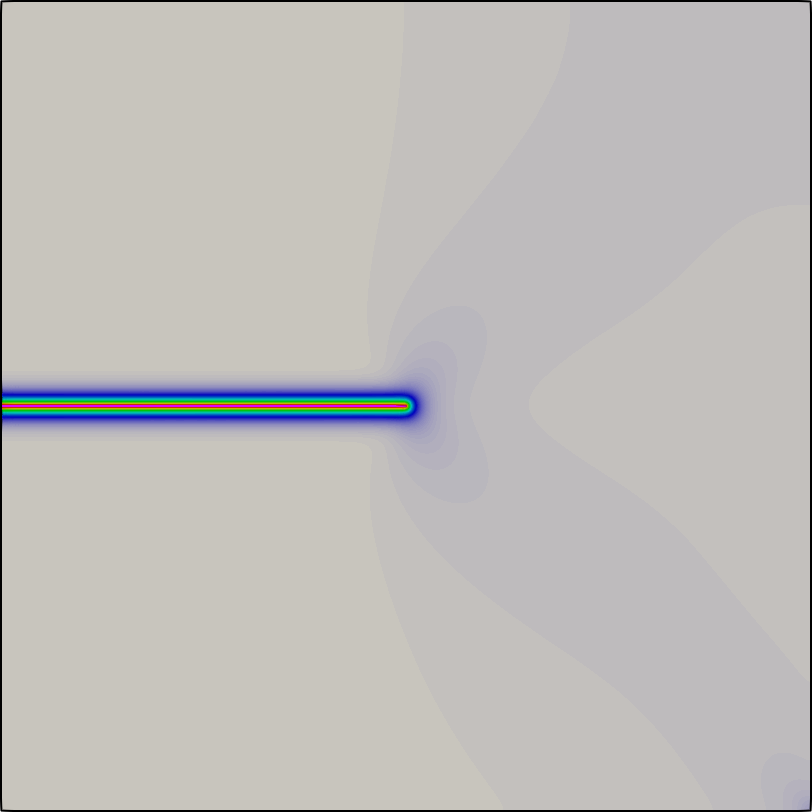
\includegraphics[scale=.1]{./Images/t30-crack.png}};
		\node at (0cm,4cm) {\scriptsize \color{black}crack~tip~(0.5,0.5)};
		\begin{axis}[
		anchor=north west,
		xshift=-1cm,yshift=11.5cm,
		enlargelimits=false,
		colorbar,
		colormap name=paraviewWR,
		point meta min=0,
		point meta max=1,
		hide axis,
		colorbar horizontal,
		colorbar style={
			ytick style={draw=none},
			xtick pos=left,
			tick align = outside,
			title style={yshift=-.28cm},
			title={damage-field~~$d$},
			scaled y ticks = false,
			height = .25cm,
			font = \scriptsize,
			width = 2.cm,
			xtick={0,0.5,1.0}
		}
		]
		\end{axis}
		\pgfplotsset{every tick label/.append style={font=\footnotesize},scaled x ticks=false}
		\begin{axis}[
		at={(0.18\linewidth,-.05\linewidth)},
		ymax=0.82,xmax=6.2e-3,
		legend style={at={(.35,.96)},anchor=north,legend columns=2,font=\fontsize{10}{5}\selectfont},
		legend image post style={scale=.9},
		xlabel={\footnotesize applied displacement~$u_2$~{[}\si{\milli\meter}{]}},
		ylabel={\footnotesize top surface force~$F_y$~{[}\si{\kilo\newton}{]}},
		xtick = { 0,2e-3,4e-3,6e-3},
		%xticklabels = { 0,2e-3,4e-3,6e-3}		
		]
		\addplot[only marks, line width=1.pt, mark=square, color=black, dotted, mark size=2pt, mark options={solid},mark repeat=2] table[x index=0, y index=1] {./Images/force-Amor-n.data};\addlegendentry{\scriptsize Amor~et~al.};
		\addplot[line width=2.pt,color=orange,mark repeat=15] table[x index=0, y index=1] {./Images/force-r1.data};\addlegendentry{\scriptsize Level 1};	
		\addplot[line width=2.pt,color=cyan,mark repeat=15] table[x index=0, y index=1] {./Images/force-r2.data};\addlegendentry{\scriptsize Level 2};		
		\addplot[line width=2.pt,color=red,mark repeat=400] table[x index=0, y index=1] {./Images/force-r3.data};\addlegendentry{\scriptsize Level 3};
		\draw[fill=black,dotted, fill opacity=.15,draw opacity=0] (axis cs:5.e-3,-1) rectangle (axis cs:6e-3,1);
		\node[rotate=90] at (axis cs:5.1e-3,0.2){\scriptsize{cracking}};	
		\node[rotate=90] at (axis cs:5.3e-3,0.2){\scriptsize{zone}};
		\end{axis}
		\node at (12.8cm,0){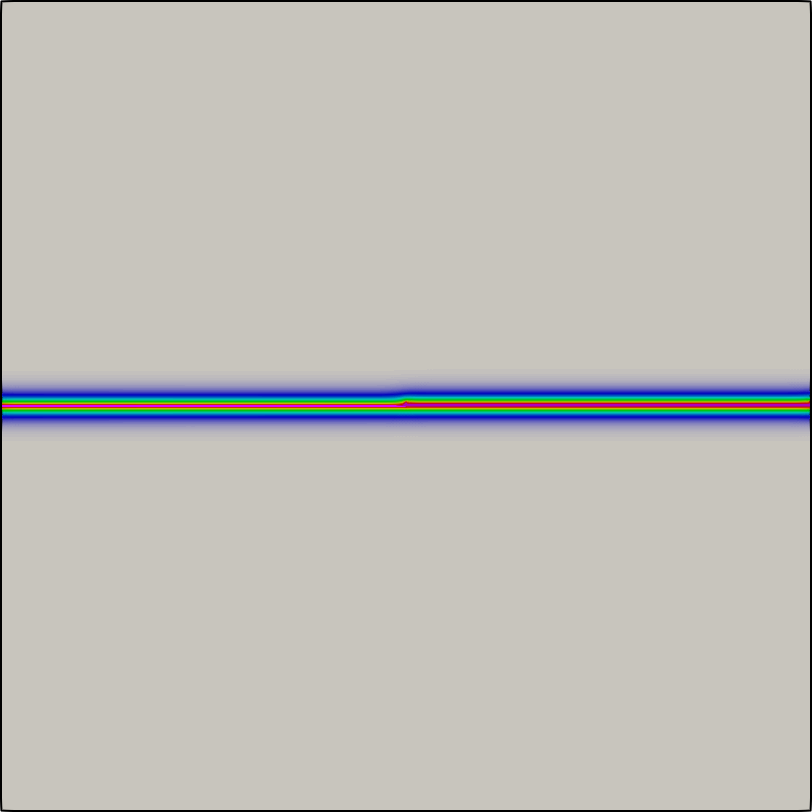
\includegraphics[scale=.1]{./Images/t141-crack.png}};
		\node at (12.8cm,0.5cm) {\scriptsize \color{black}crack~tip~(1.0,0.5)};
		\node at (12.8cm,3.25cm){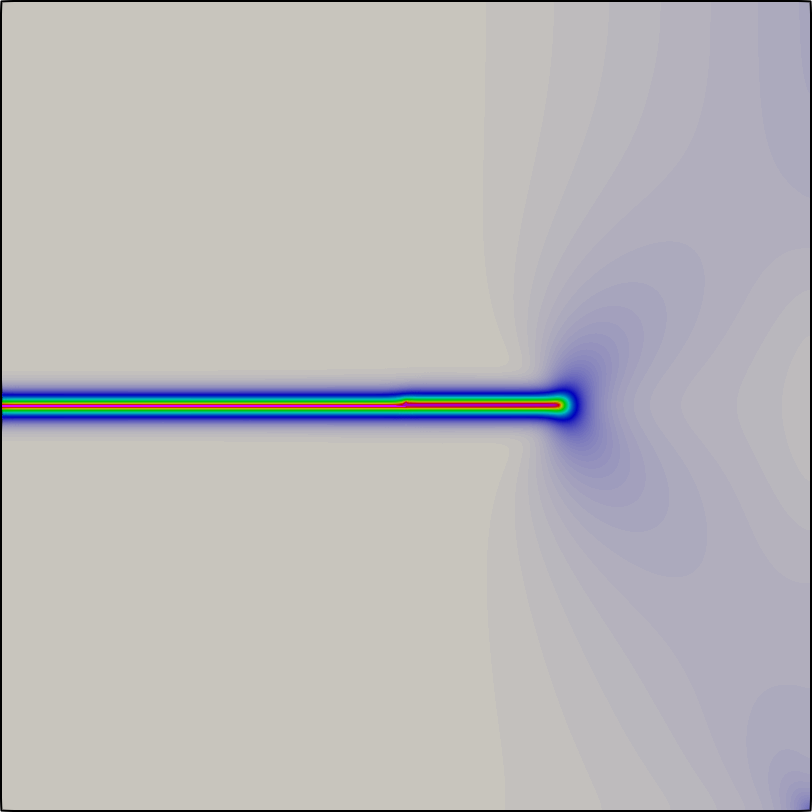
\includegraphics[scale=.1]{./Images/t101-crack.png}};
		\node at (12.8cm,4cm) {\scriptsize \color{black}crack~tip~(0.7,0.5)};
		\begin{axis}[
		at={(12.8cm,0)},
		anchor=north west,
		xshift=-1cm,yshift=11.5cm,
		enlargelimits=false,
		colorbar,
		colormap name=paraviewWR,
		point meta min=0,
		point meta max=1,
		hide axis,
		colorbar horizontal,
		colorbar style={
			ytick style={draw=none},
			xtick pos=left,
			tick align = outside,			
			title style={yshift=-.28cm},
			title={damage-field~~$d$},
			scaled y ticks = false,
			height = .25cm,
			font = \scriptsize,
			width = 2.cm,
			xtick={0,0.5,1.0}
		}
		]
		\end{axis}
		\draw[black,thick,dashed] (1.5,0) -- (2.5,0) -- (3.5,-.3);
		\draw[black,thick,dashed] (1.5,4) -- (2.5,4) -- (6,1.8);
		\draw[black,thick,dashed] (11.35,0) -- (10.35,0) -- (9.4,-.2);
		\draw[black,thick,dashed] (11.35,4) -- (10.35,4)  -- (9.3,1.6);;
		\end{tikzpicture}
	\end{minipage}
	\caption{mesh convergence demonstrated via force-displacement plot for the two-dimensional single-edge notched tensile fracture simulation, test~1. The solid lines (Level 1 to 3) refers to our PSD solution for different mesh refinements and the square markers denote the reference solution (obtained by the anisotropic phase-field method) presented by~\cite{amor2009regularized}.\label{fig:force-comp-2d-tensile-crack}}
\end{figure}

\section{Validating the PSD soil-dynamic solver with paraxial boundary conditions}
In this subsection we would compare the paraxial absorbing elements implemented in PSD against other absorbing boundary conditions available in CAST3M\footnote{The CAST3M numerical experiments are performed by Reine Fares - Research Engineer - CEA/SEMT.}. This document also serves as a naive cross validation of the PSD solvers parallel/sequential kernel developed for soil-dynamics.

\subsection{Numerical experiment 1: A two-dimensional square}
The geometry is considered to be a square with 50 m side, meshed with 1 m elements. This test is inspired by the validation tests performed in the paper of Bambeger et al.~1988. The paraxial conditions (resp.~absorbing boundary conditions)  apply to the bottom, left, and right borders for the PSD simulation (resp.~for the CAST3M simulation). \Cref{fig:geo} illustrates the geometry, red borders depict the absorbing (paraxial) borders and the green one depicts the free boundary condition. 

\begin{figure}[htbp]
	\centering
	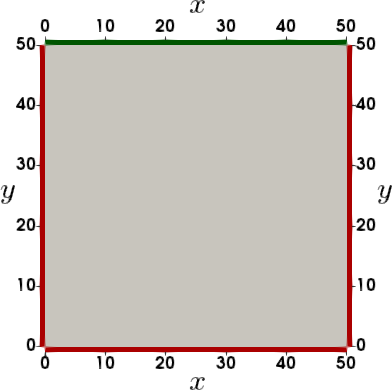
\includegraphics[width=.3\textwidth]{./Images/geo.png}
	\caption{The two-dimensional geometry with paraxial borders in red and the free field border in green.\label{fig:geo}}
\end{figure}

\noindent The essential algorithmic  parameters concerning time discretization are enlisted below, while the material properties are tabulated in~\cref{tab:material-properties}.    
\begin{itemize}

\item Time step used for the generalized-$\alpha$ scheme is $\text{d}t=0.01$~sec 

\item The generalized-$\alpha$ parameters read $\alpha_m=0.0$ and $\alpha_f=0.0$. Note that these null values for $\alpha_m$ and $\alpha_f$ transforms the generalized-$\alpha$ time discretization scheme into a Newmark-$\beta$ time discretization scheme. Hence, a  Newmark-$\beta$ is used  both in PSD and CAST3M.

\item The simulation is run for $t=4.0$ seconds, hence requiring 400 iterations of  the solver.   		
\end{itemize}





{
	\pgfplotstableread{
		A			B			C       D           
		Test~1	 2500		6.62E6    	0.45	
		
	}\datatab 
	\begin{table}[htbp]\centering
		\pgfplotstabletypeset[
		font=\footnotesize,
		columns={A,B,C,D},
		columns/A/.style={column name =Case,string type,column type = {l}},
		columns/B/.style = {column name =$\rho$~[\si{\kilogram\per\cubic\meter}],string type,precision =0,fixed zerofill,column type = {l}},
		columns/C/.style = {column name =$E$~[\si{\pascal}],string type,precision =0,fixed zerofill,column type = {l}},
		columns/D/.style = {column name =$\nu$,string type,fixed zerofill,column type = {r}},
		every odd row/.style={before row={\rowcolor{white}}},
		every even row/.style={before row={\rowcolor{black!9}}},
		every head row/.style={before row={\midrule},after row=\midrule},
		every last row/.style={after row=\midrule},
		]{\datatab}
		\caption{ Parameters for the seismic test.   \label{tab:material-properties}}
	\end{table}
}


Before proceeding to the simulation comparison it is notified that meshes used by PSD and CASTEM, are triangular and quard type, respective. \Cref{fig:meshes} illustrates the difference between the PSD and the CASTEM meshes.

\begin{figure}[h]
	\centering
	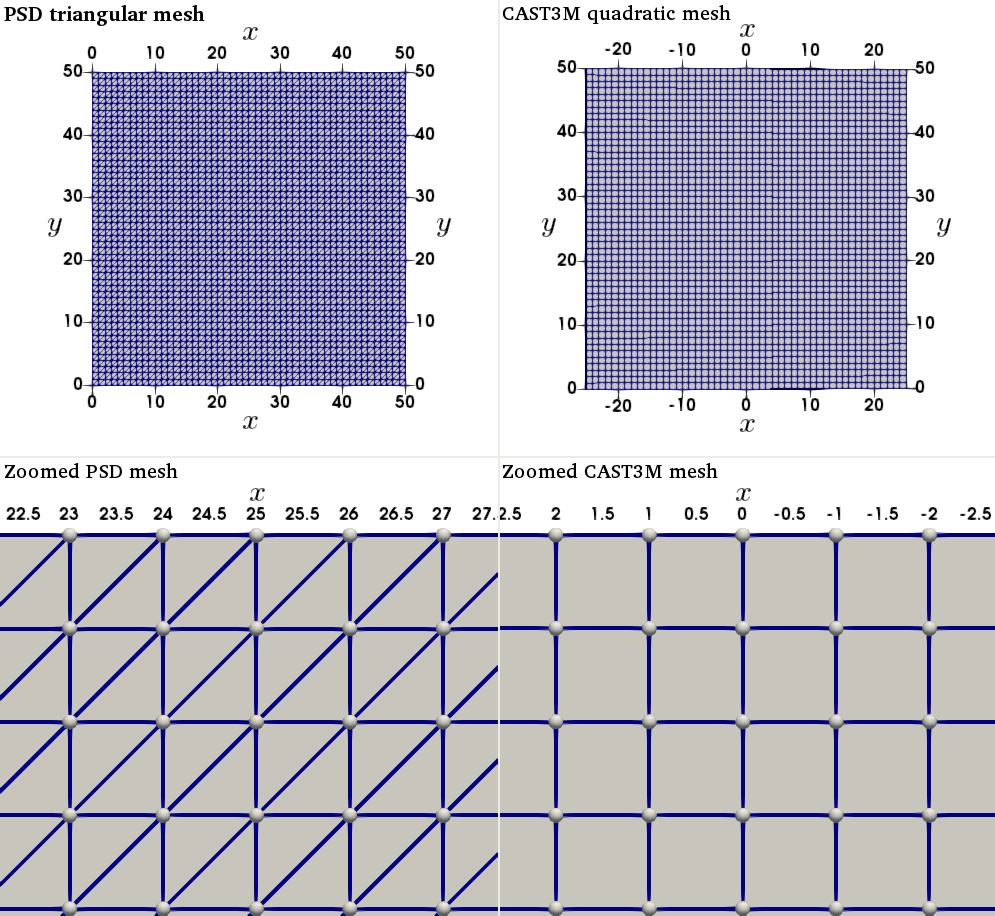
\includegraphics[width=.8\textwidth]{./Images/mesh-CAST3M-PSD}
	\caption{Meshes used by CAST3M (right) and PSD (left).\label{fig:meshes} }
\end{figure}

\subsection{Test 1: top loading of the square}
We test how the solvers behave when the free boundary is loaded. 

\begin{itemize}
	\item Concerning the loading, on the center region of the top border we apply a small sinusoidal excitation spread over 1  seconds. The applied force reads:
	$$\int_{\partial \Omega} (\sigma\cdot\textbf{n})\cdot\bv  = \int_{\partial \Omega} \left(\rho c_{\text{p}}\left( \sin(2\pi t\big /1.0)\right)\mathbbm{1}_{[x>20~~\&~~x<30~~\&~~y=50  ]}\times\mathbbm{1}_{[t\le1]}\right)v_1$$
	
		 	
\end{itemize}



\subsection{Test 2: bottom loading of the square}
We test how the solvers behave when one of the paraxial (absorbing) boundary is loaded. 

\begin{itemize}
	\item Concerning the loading, on the center region of the bottom border we apply a small sinusoidal excitation spread over 1  seconds. The applied force reads:
	$$\int_{\partial \Omega} (\sigma\cdot\textbf{n})\cdot\bv  = \int_{\partial \Omega} \left(\rho c_{\text{p}}\left( \sin(2\pi t\big /1.0)\right)\mathbbm{1}_{[x>20~~\&~~x<30~~\&~~y=0]}\times\mathbbm{1}_{[t\le1]}\right)v_1$$
	
	
\end{itemize}


   

\begin{figure}[h]
	\centering
	\begin{tikzpicture}
	\begin{axis}[height=8cm,width=17cm,
	%xmin=0.0008, xmax=.015,
	%ymin=1e-9, ymax=1e-5,
	mark repeat={1},
	legend style={at={(.5,1.22)},anchor=north,legend columns=2,font=\fontsize{10}{5}\selectfont},
	legend image post style={scale=.9},
	%xtick = {.01, .005, .0025, .00125},
	%xticklabels = {0.01, 0.005, 0.0025, 0.00125},
	xlabel={Time (s)},
	ylabel={Y- Velocity (m/s)}
	]
	\addplot[ line width=1.pt, mark=square, color=blue, mark size=1.5pt] table[x index=0, y index=1] {./Images/Cast3m-upper.data};\addlegendentry{CAST3M};		
	\addplot[ mark=*, color=orange, mark size=1.5pt, mark options={solid}] table[x index=0, y index=1] {./Images/PSD-upper.data};\addlegendentry{PSD};
			
	
	\end{axis}
	\end{tikzpicture}
	\caption{Test 1 results. Comparison of Y-velocities of a point $\bx=(25,50)$ obtained by CAST3M and PSD for a 4 second simulation with 1 second sinusoidal wave excitation.  }\label{fig:top}
\end{figure}

\begin{figure}[h]
	\centering
	\begin{tikzpicture}
	\begin{axis}[height=8cm,width=17cm,
	%xmin=0.0008, xmax=.015,
	%ymin=1e-9, ymax=1e-5,
	mark repeat={1},
	legend style={at={(.5,1.22)},anchor=north,legend columns=2,font=\fontsize{10}{5}\selectfont},
	legend image post style={scale=.9},
	%xtick = {.01, .005, .0025, .00125},
	%xticklabels = {0.01, 0.005, 0.0025, 0.00125},
	xlabel={Time (s)},
	ylabel={Y- Velocity (m/s)}
	]

	
	\addplot[ line width=1.pt, mark=square, color=blue, mark size=1.5pt] table[x index=0, y index=1] {./Images/Cast3m-lower.data};\addlegendentry{CAST3M};		
	\addplot[ mark=*, color=orange, mark size=1.5pt, mark options={solid}] table[x index=0, y index=1] {./Images/PSD-lower.data};\addlegendentry{PSD};
			
	
	\end{axis}
	\end{tikzpicture}
	\caption{Test 1 results. Comparison of Y-velocities of a point $\bx=(25,0)$ obtained by CAST3M and PSD for a 4 second simulation with 1 second sinusoidal wave excitation.  }\label{fig:bottom}
\end{figure}


\begin{figure}
	\centering
	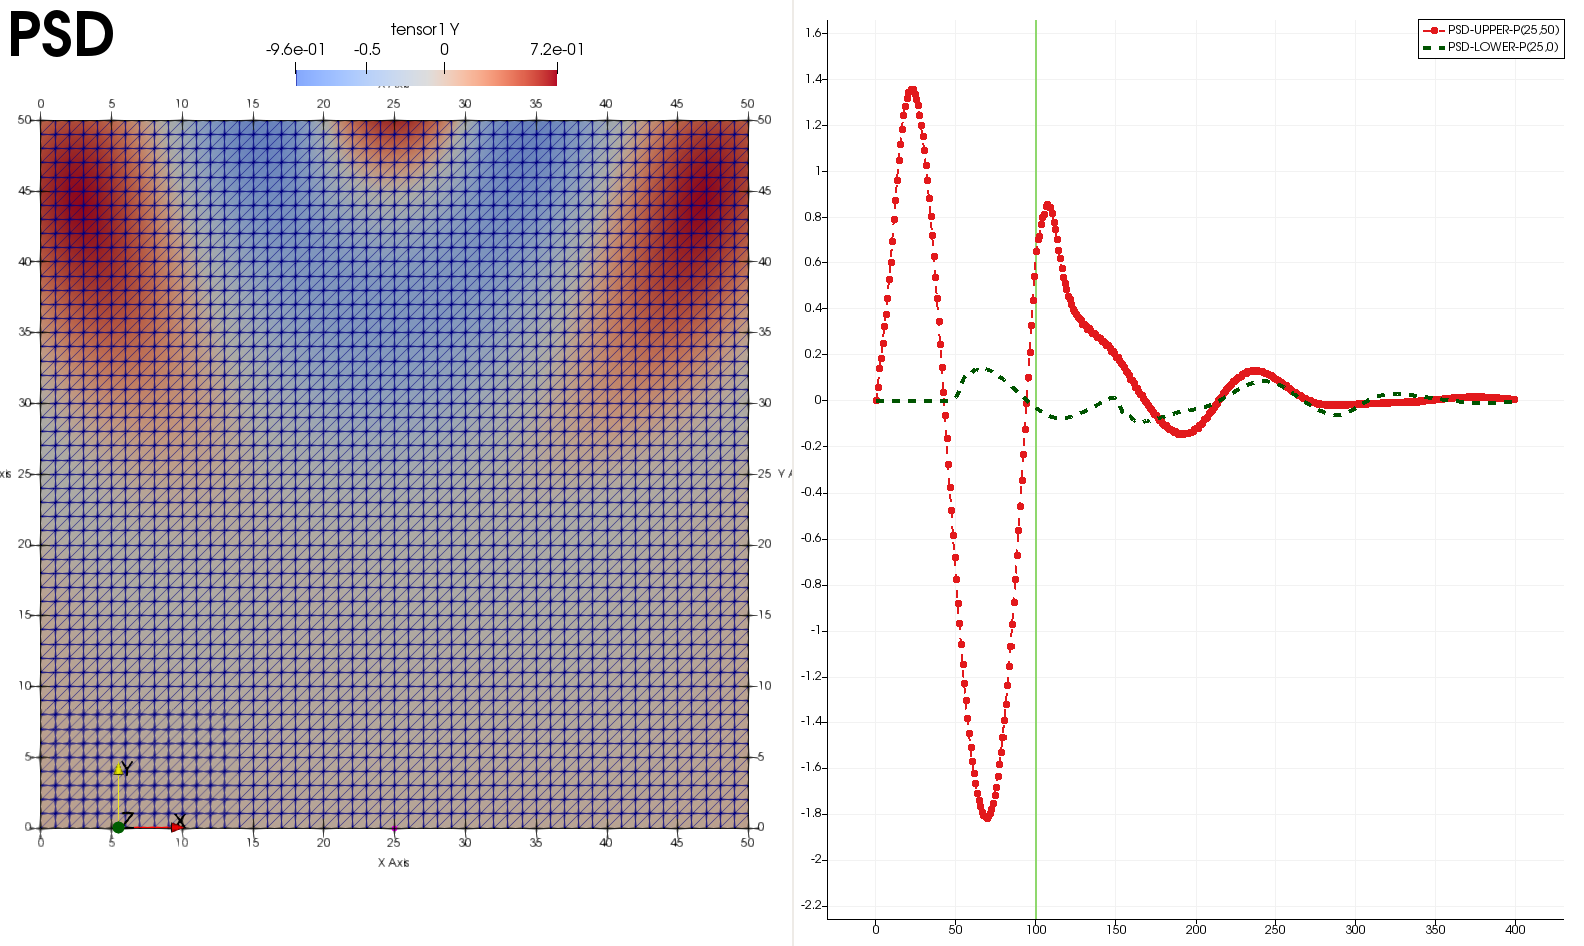
\includegraphics[width=.8\textwidth]{./Images/PSD-t1}\\\vspace{1cm}
	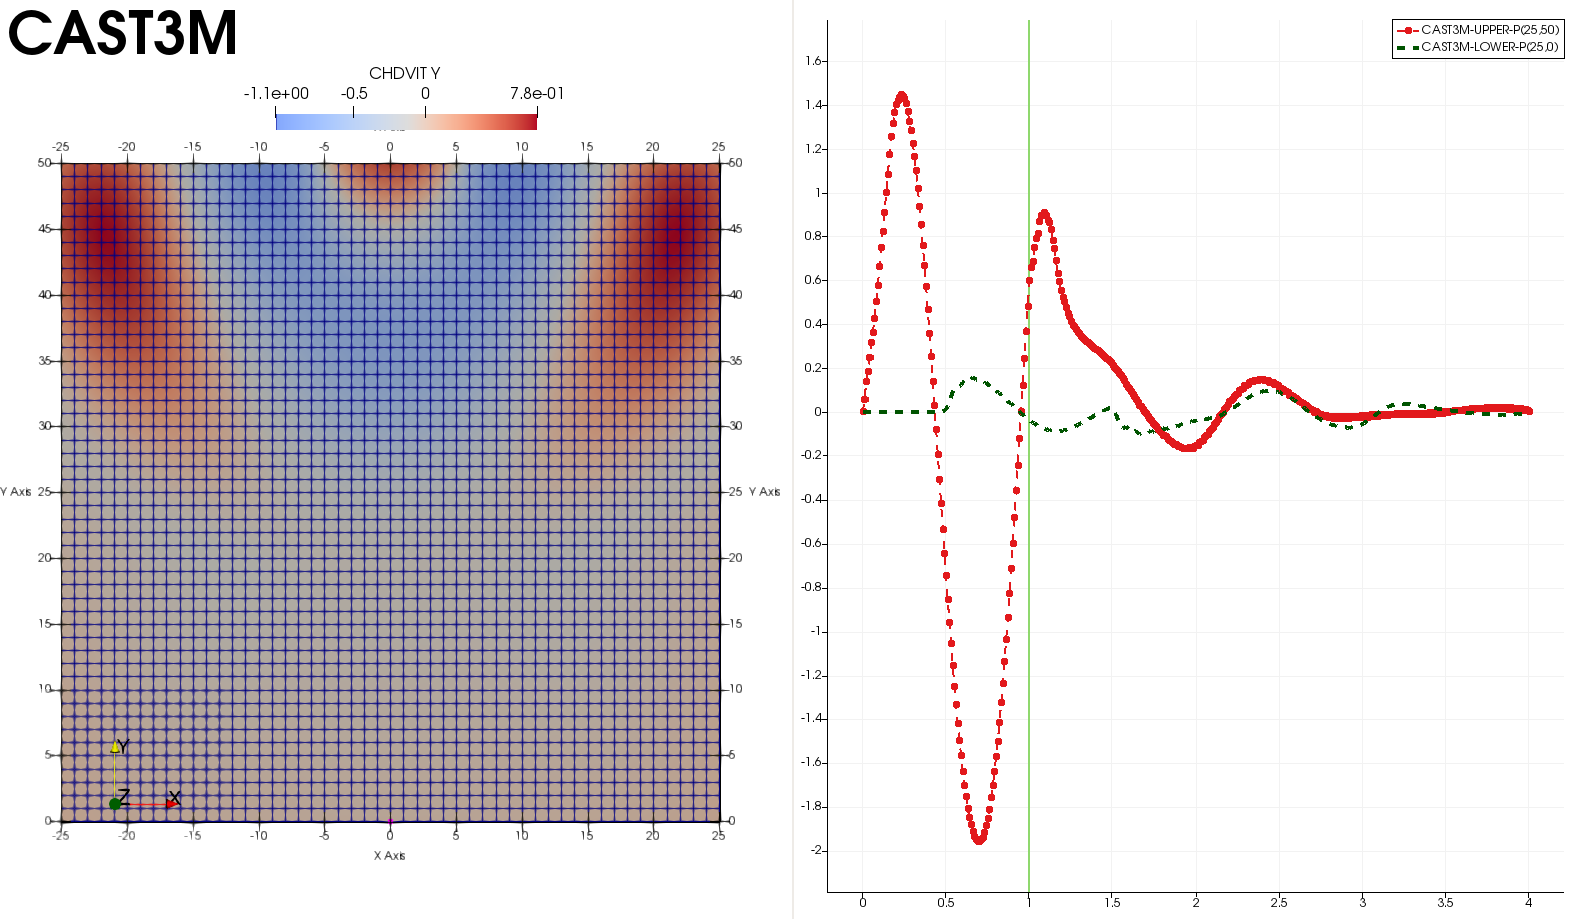
\includegraphics[width=.8\textwidth]{./Images/CAST3M-t1}
	\caption{Comparison of simulations performed  in CAST3M and PSD. Left: Y-velocity field snapshot at $t=1.0$~second. Right: Top and bottom border point ($x=25$) time history for Y-velocities.   }\label{fig:CastemPSD1}
\end{figure}


\begin{figure}
	\centering
	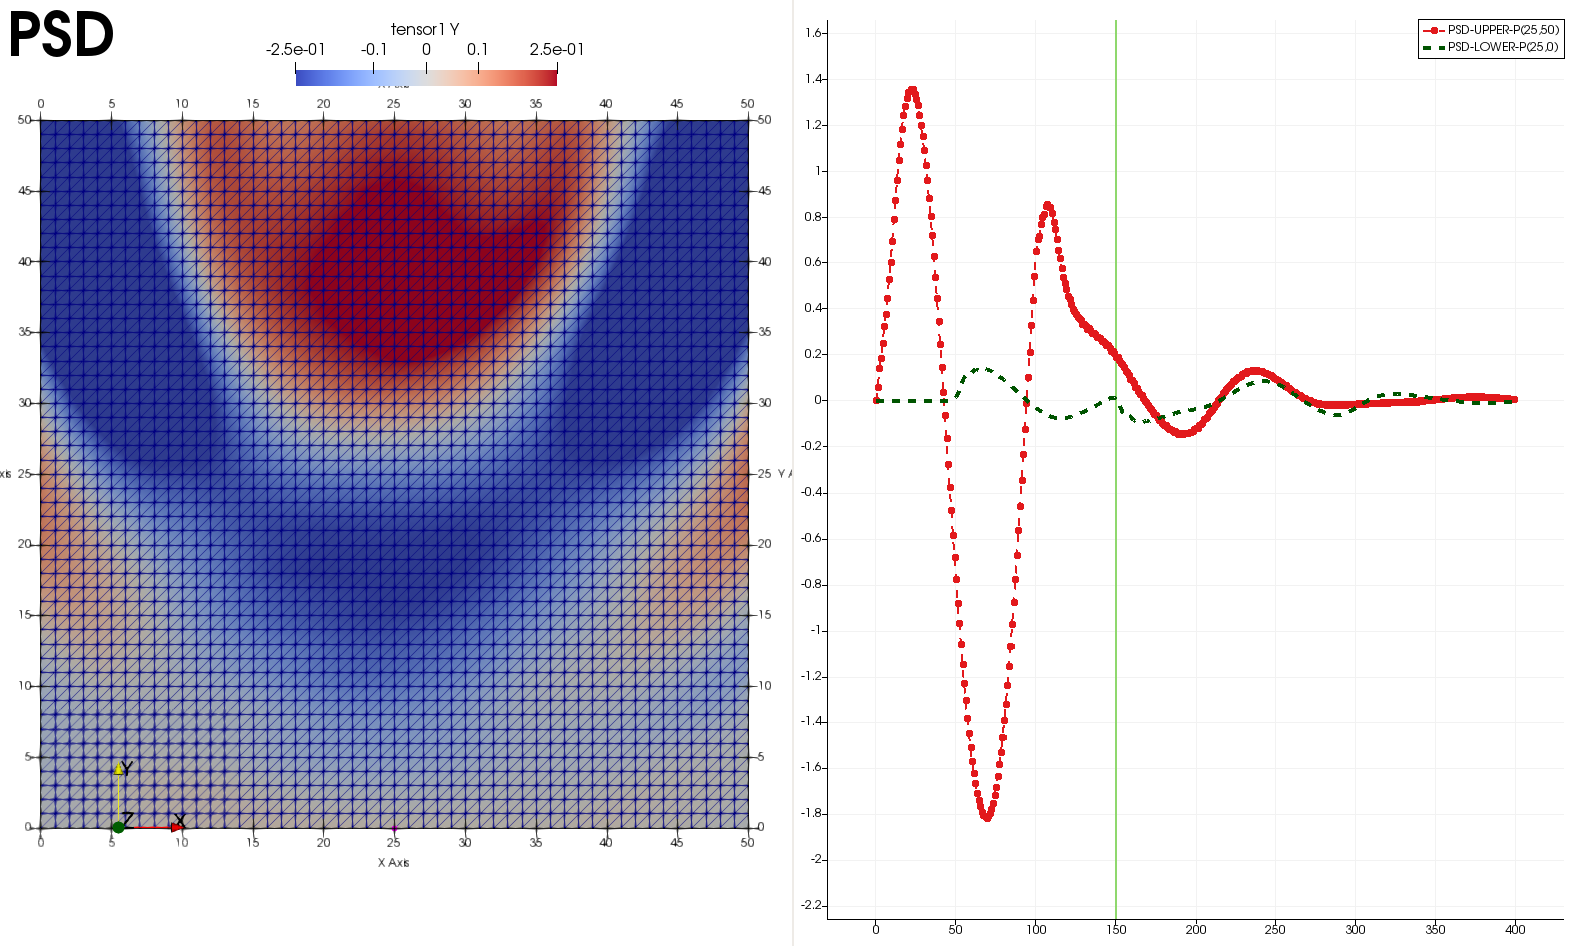
\includegraphics[width=.8\textwidth]{./Images/PSD-t2}\\\vspace{1cm}
	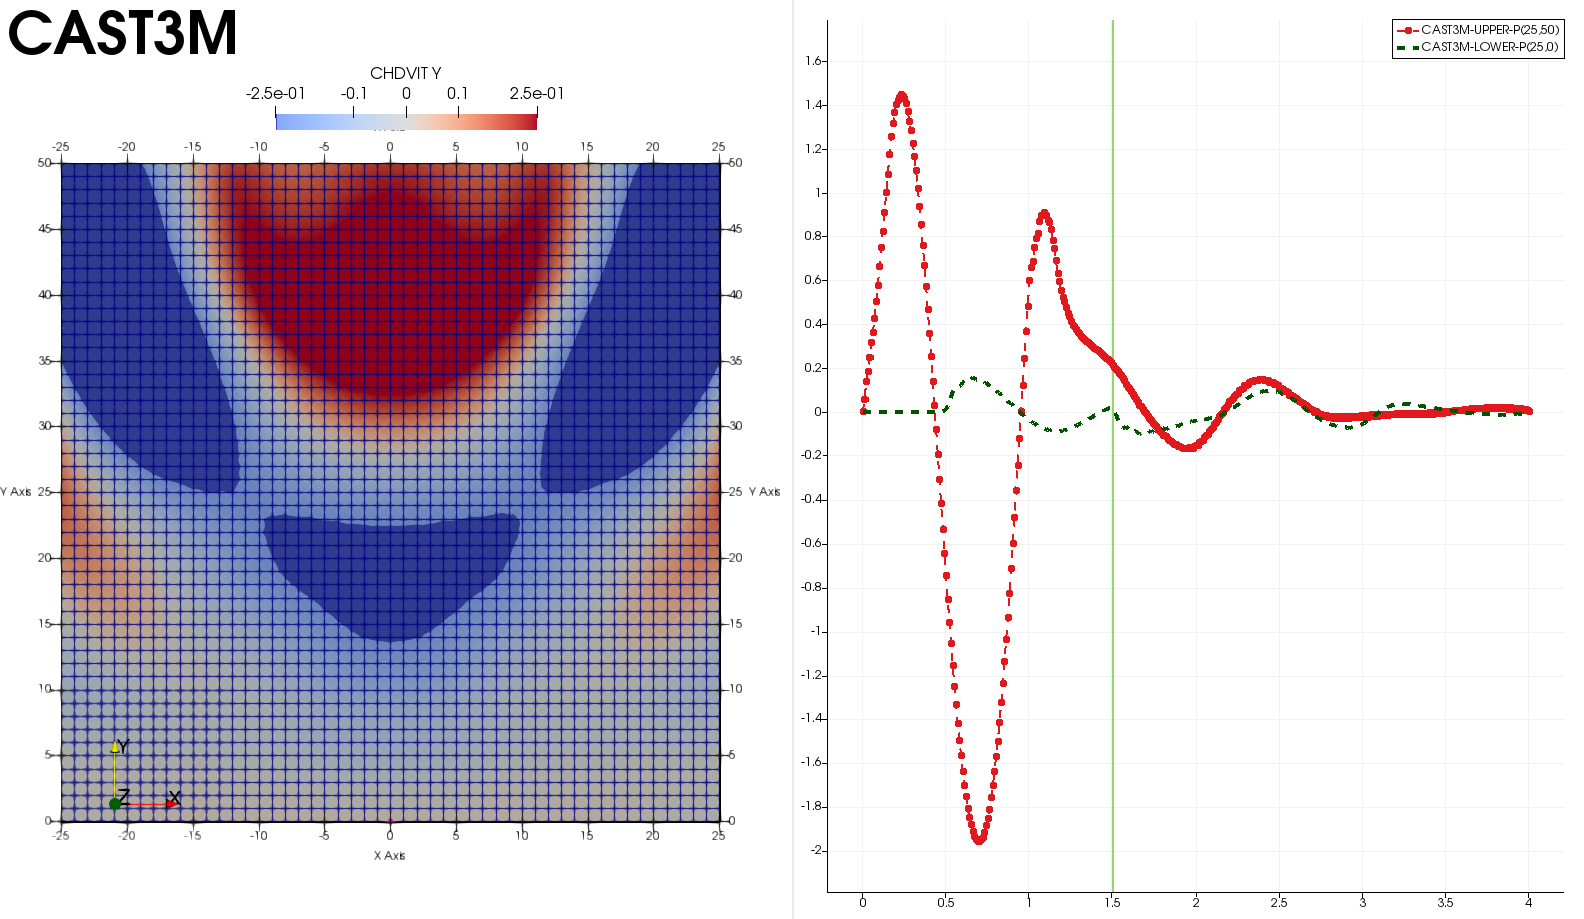
\includegraphics[width=.8\textwidth]{./Images/CAST3M-t2}
	\caption{Comparison of simulations performed  in CAST3M and PSD. Left: Y-velocity field snapshot at $t=1.5$~second. Right: Top and bottom border point ($x=25$) time history for Y-velocities.   }\label{fig:CastemPSD2}
\end{figure}


\begin{figure}
	\centering
	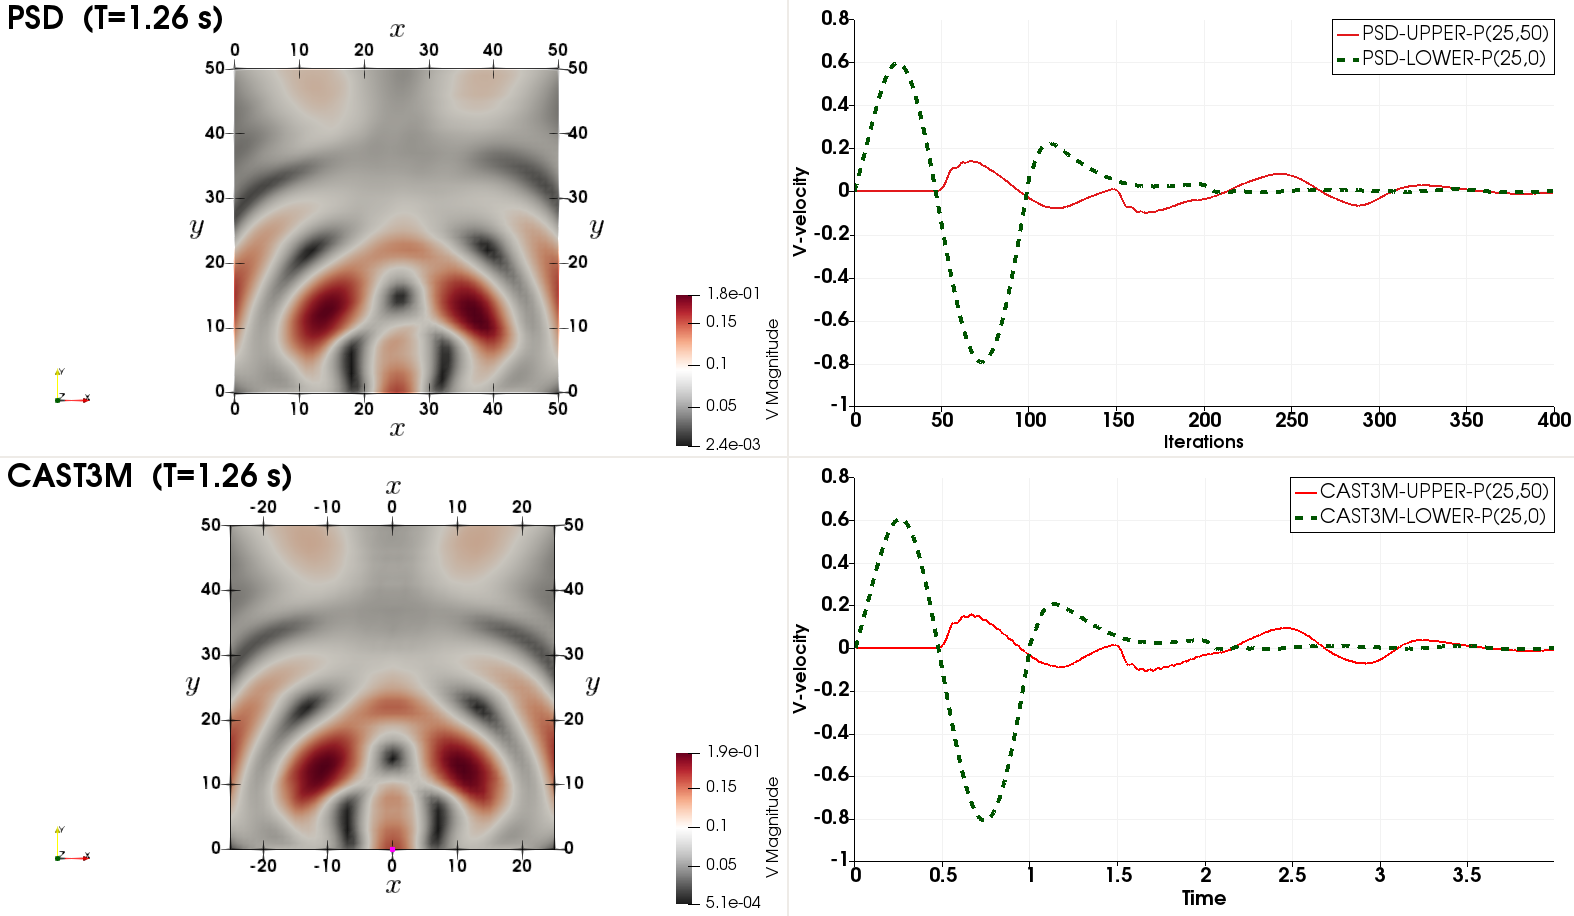
\includegraphics[width=.8\textwidth]{./Images/Test2-CAST3M-Vs-PSD.png}
	\caption{Comparison of simulations performed  in CAST3M and PSD. Left: Y-velocity field snapshot at $t=1.26$~second. Right: Top and bottom border point ($x=25$) time history for Y-velocities.   }\label{fig:CastemPSD2-test2}
\end{figure}


\begin{figure}[h]
	\centering
	\begin{tikzpicture}
	\begin{axis}[height=8cm,width=17cm,
	%xmin=0.0008, xmax=.015,
	%ymin=1e-9, ymax=1e-5,
	mark repeat={1},
	legend style={at={(.5,1.22)},anchor=north,legend columns=2,font=\fontsize{10}{5}\selectfont},
	legend image post style={scale=.9},
	%xtick = {.01, .005, .0025, .00125},
	%xticklabels = {0.01, 0.005, 0.0025, 0.00125},
	xlabel={Time (s)},
	ylabel={Y- Velocity (m/s)}
	]
	\addplot[ line width=1.pt, mark=square, color=blue, mark size=1.5pt] table[x index=0, y index=1] {./Images/CAST3M-TOP.csv};\addlegendentry{CAST3M};		
	\addplot[ mark=*, color=orange, mark size=1.5pt, mark options={solid}] table[x index=0, y index=1] {./Images/PSD-TOP.csv};\addlegendentry{PSD};
	
	
	\end{axis}
	\end{tikzpicture}
	\caption{Test 2 results. Comparison of Y-velocities of a point $\bx=(25,50)$ obtained by CAST3M and PSD for a 4 second simulation with 1 second sinusoidal wave excitation.  }\label{fig:top1}
\end{figure}

\begin{figure}[h]
	\centering
	\begin{tikzpicture}
	\begin{axis}[height=8cm,width=17cm,
	%xmin=0.0008, xmax=.015,
	%ymin=1e-9, ymax=1e-5,
	mark repeat={1},
	legend style={at={(.5,1.22)},anchor=north,legend columns=2,font=\fontsize{10}{5}\selectfont},
	legend image post style={scale=.9},
	%xtick = {.01, .005, .0025, .00125},
	%xticklabels = {0.01, 0.005, 0.0025, 0.00125},
	xlabel={Time (s)},
	ylabel={Y- Velocity (m/s)}
	]
	
	
	\addplot[ line width=1.pt, mark=square, color=blue, mark size=1.5pt] table[x index=0, y index=1] {./Images/CAST3M-BOT.csv};\addlegendentry{CAST3M};		
	\addplot[ mark=*, color=orange, mark size=1.5pt, mark options={solid}] table[x index=0, y index=1] {./Images/PSD-BOT.csv};\addlegendentry{PSD};
	
	
	\end{axis}
	\end{tikzpicture}
	\caption{Test 2 results. Comparison of Y-velocities of a point $\bx=(25,0)$ obtained by CAST3M and PSD for a 4 second simulation with 1 second sinusoidal wave excitation.  }\label{fig:bottom1}
\end{figure}


{
	\pgfplotstableread{
		A			B			C       D    	E       
		PSD		sequential		96    	Test~1	paraxial
		PSD		sequential-opt.	45		Test~1  paraxial
		PSD		parallel		9		Test~1	paraxial
		CAST3M	sequential		180 	Test~1	Lysmer-type	
		
	}\datatab 
	\begin{table}[htbp]\centering
		\pgfplotstabletypeset[
		font=\footnotesize,
		columns={D,A,B,C,E},
		columns/A/.style={column name =package,string type,column type = {l}},
		columns/B/.style = {column name =version,string type,precision =0,fixed zerofill,column type = {l}},
		columns/C/.style = {column name =time,string type,precision =0,fixed zerofill,column type = {l}},
		columns/D/.style = {column name =Case,string type,fixed zerofill,column type = {r}},
		columns/E/.style = {column name =boundary,string type,fixed zerofill,column type = {l}},		
		every odd row/.style={before row={\rowcolor{white}}},
		every even row/.style={before row={\rowcolor{black!9}}},
		every head row/.style={before row={\midrule},after row=\midrule},
		every last row/.style={after row=\midrule},
		]{\datatab}
		\caption{ CPU time comparison of CAST3M and PSD for different test/versions.  CPU time is given in seconds, PSD version sequential-opt.~means PSD with the  GFP library (GoFastPlugins), by default the GFP library is used for PSD parallel version. As the mesh is tiny, only 4 MPI processes are used in the PSD parallel version.   \label{tab:packages}}
	\end{table}
}

\begin{figure}
	\centering
	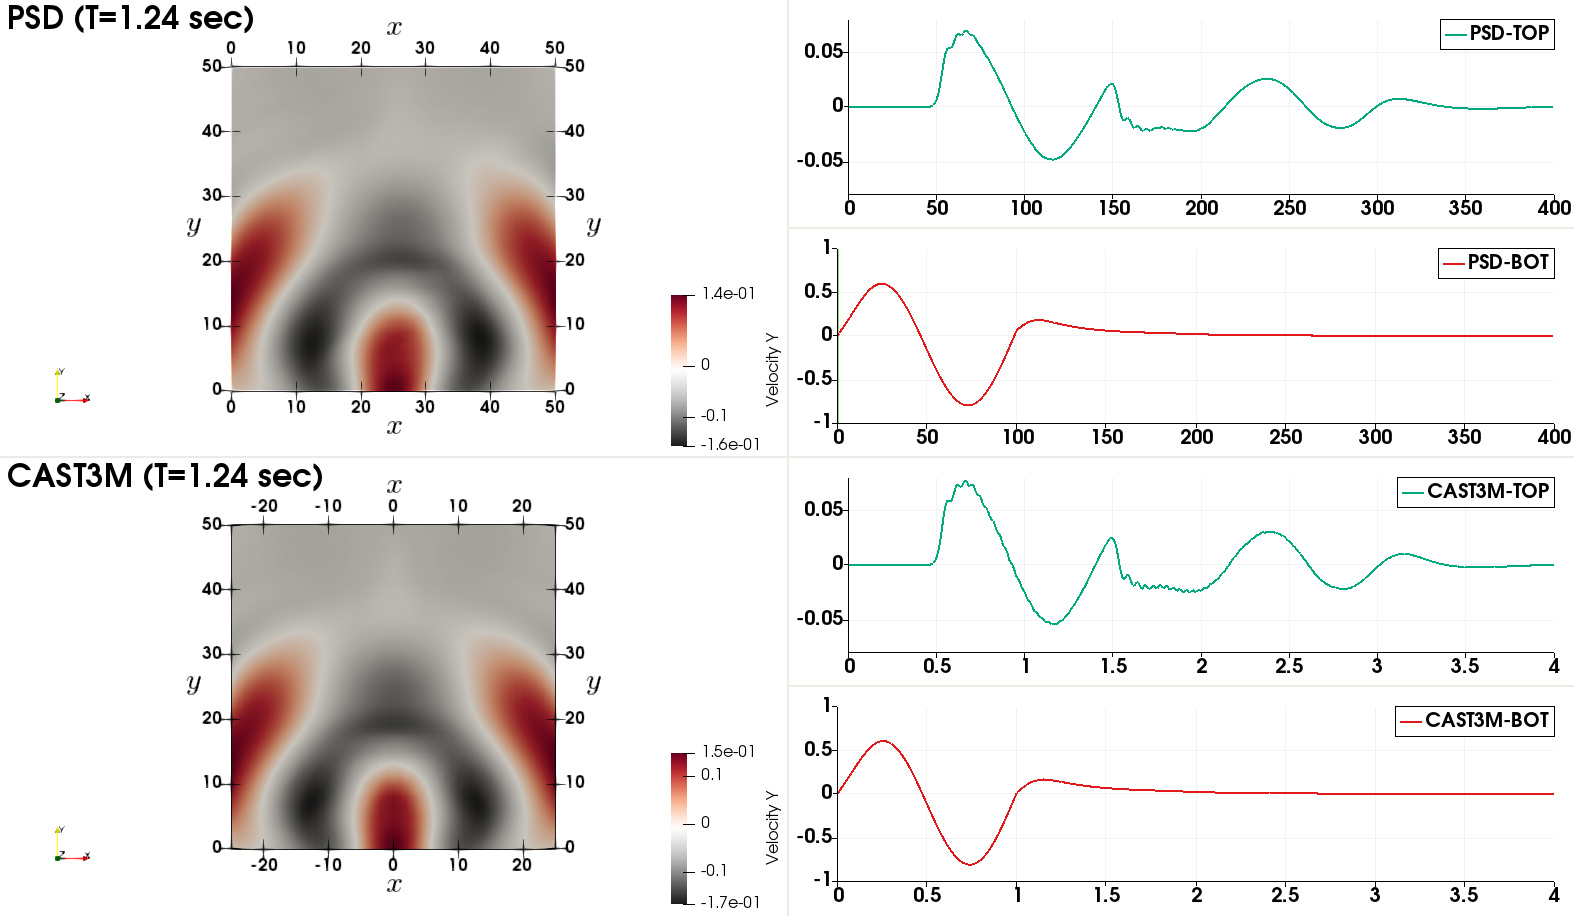
\includegraphics[width=.8\textwidth]{./Images/Test3-CAST3M-Vs-PSD.png}
	\caption{Comparison of simulations performed  in CAST3M and PSD. Left: Y-velocity field snapshot at $t=1.26$~second. Right: Top and bottom border point ($x=25$) time history for Y-velocities.   }\label{fig:CastemPSD2-test3}
\end{figure}

\subsection{Numerical experiment 2: 3D case with complex geometry}

\begin{figure}
    \centering
    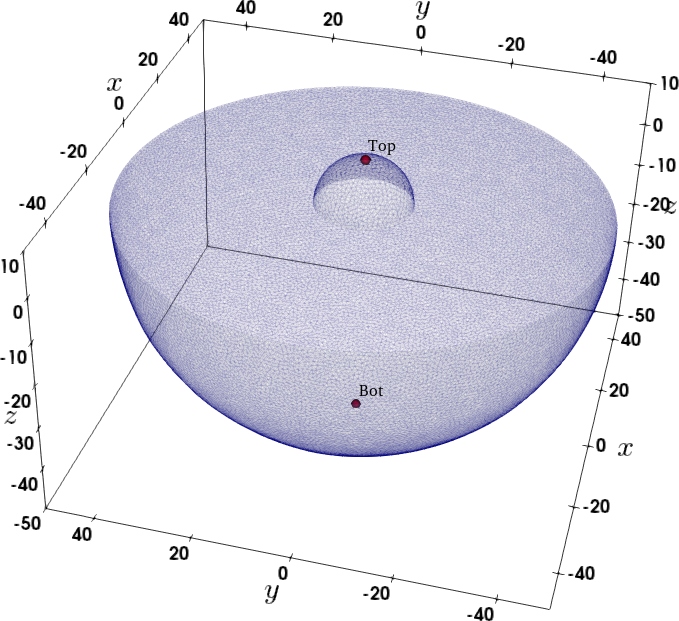
\includegraphics[width=0.45\textwidth]{./Images/top-bot.png}        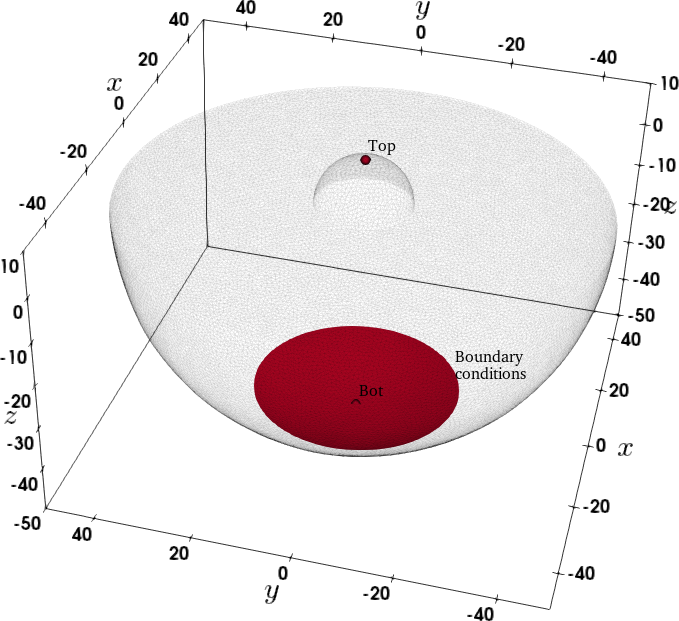
\includegraphics[width=0.45\textwidth]{./Images/top-bot-bc.png}\\
    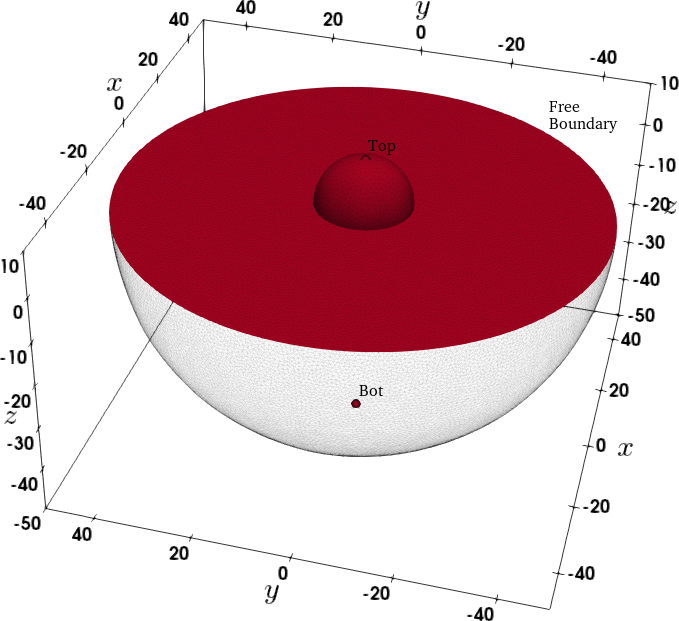
\includegraphics[width=0.45\textwidth]{./Images/top-bot-bc1.png}        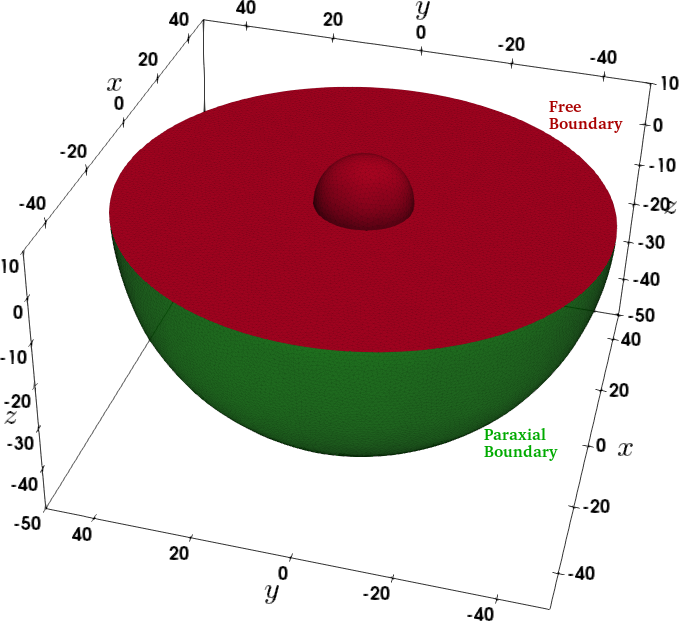
\includegraphics[width=0.45\textwidth]{./Images/top-bot-bc2.png}\\
    \caption{Seismic 3D cased with complex geometry and boundary conditions.}
    \label{fig:soilsemiCastemPSD3D}
\end{figure}

\begin{figure}
	\centering
	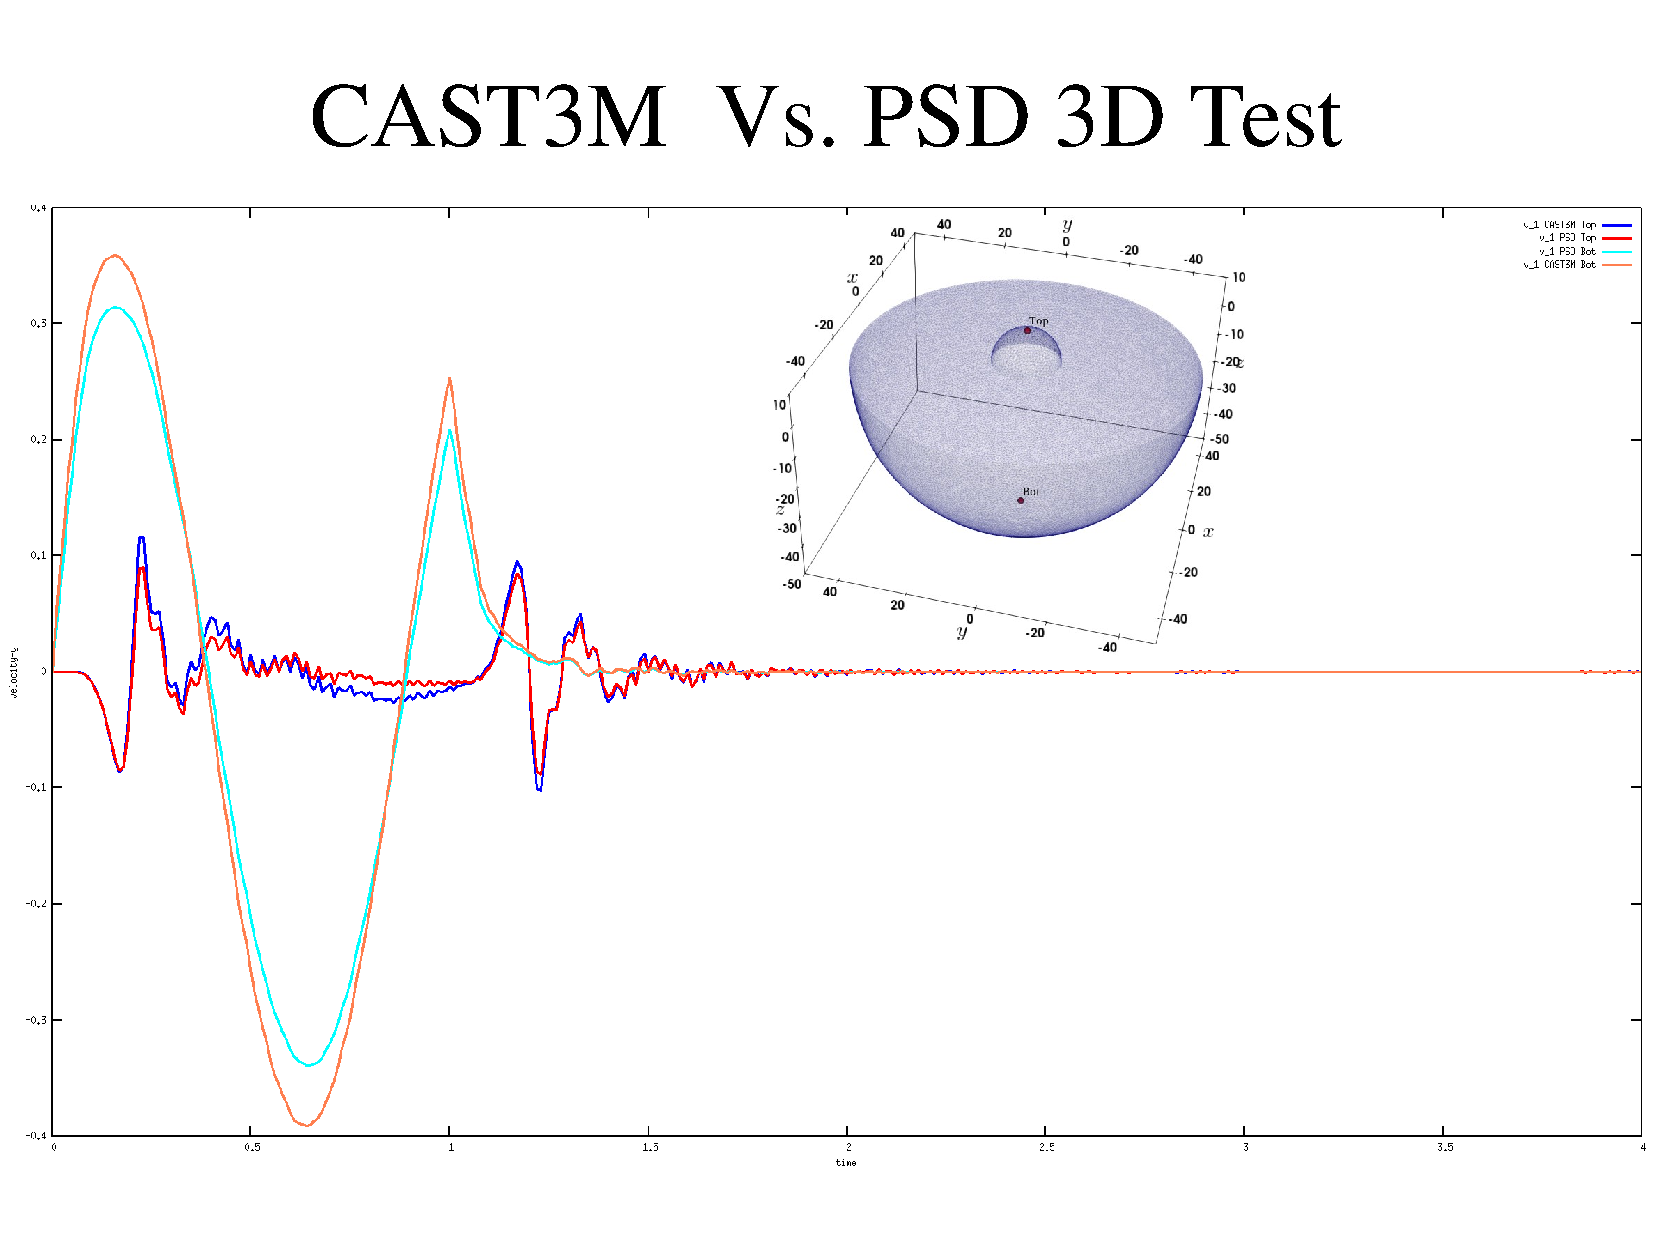
\includegraphics[width=.85\textwidth]{./Images/Cast3MPSD.pdf}
	\caption{Comparison of 3D simulations performed  in CAST3M and PSD.   }\label{fig:CastemPSD3D}
\end{figure}
